\subsubsection{\warpunit}

%
A {\warpunit} generally consists of the following 5 gadgets: {\prewarp}, {\firstwarp}, {\warpbridge}, {\secondwarp}, and {\postwarp}.
%
The job of these 5 gadgets is to transport the value read by the {\cread} all the way to the digit region in the next row, so that the {\cwrite} gadgets can write the next value in the correct locations.
%


\begin{itemize}

    \item {\prewarp}:
    %
    These gadgets decode the least significant two bits passed in from the read {\cread} gadgets into a special signal that indicates whether a gadget is currently in the MSR, and if it is, whether it is also the MSD.
    %
    Here is how the signal is decoded: if the least significant bit is 1, add a marker to indicate the current gadgets are in the MSR; if the second least significant bit is also 1, add a marker on the glues to indicate that the gadget is also part of the MSD.

    For each $i = 1,2,3, u \in \{0, 1\}^l$, and each $\inc \in \ops$:
    \begin{itemize}
        \item if $u$ ends with 00:
        create
        $\begin{aligned}[t]
            \prewarp(& \left\langle {\tt PreWarp},   i, u, \inc \right\rangle,
                       \left\langle {\tt FirstWarp}, i, u, \inc \right\rangle \;)
        \end{aligned}$ \\ from the general gadget in Figure~\ref{fig:pre_warp_general}.

        \item if $u$ ends with 01:
        $\begin{aligned}[t]
            \prewarp(& \left\langle {\tt PreWarp},   1, u, \inc            \right\rangle,
                       \left\langle {\tt FirstWarp}, 1, u, \inc, {\tt msr} \right\rangle \;)
        \end{aligned}$ \\ from the general gadget in Figure~\ref{fig:pre_warp_1_op_msr_msd}.

        \item if $u$ ends with 11:
        create
        $\begin{aligned}[t]
            \prewarp(& \left\langle {\tt PreWarp},   i, u, \inc                       \right\rangle,
                       \left\langle {\tt FirstWarp}, i, u, \inc, {\tt msr}, {\tt msd} \right\rangle \;)
        \end{aligned}$ from the general gadget in Figure~\ref{fig:pre_warp_1_op_msr} if $i = 1$ (case 1),
        or Figure~\ref{fig:pre_warp_2_op_msr_msd} if $i = 2$ (case 2), or Figure~\ref{fig:pre_warp_general} if $i = 3$ (case 3).
    \end{itemize}
    \vspace{.5cm}

    In this step, for digits 1-3 in the general case,
    %
    $9 \cdot 2^l \cdot 34 =$
    %
    $306 \cdot 2^l =$
    %
    $306 \cdot 2^{\ceil*{{\log m}} + 2} =$
    %
    $1224 \cdot 2^{\ceil*{\log m}} \leq$
    %
    $2448 \cdot 2^{\log m} = \bigom$ tiles were created.
    %

    For digit 1 in case 1,
    %
    $3 \cdot 2^l \cdot 31 =$
    %
    $93 \cdot 2^l =$
    %
    $93 \cdot 2^{\ceil*{{\log m}} + 2} =$
    %
    $372 \cdot 2^{\ceil*{\log m}} \leq$
    %
    $744 \cdot 2^{\log m} = \bigom$ tiles were created.
    %

    For digit 1 in case 2,
    %
    $3 \cdot 2^l \cdot 34 =$
    %
    $102 \cdot 2^l =$
    %
    $102 \cdot 2^{\ceil*{{\log m}} + 2} =$
    %
    $408 \cdot 2^{\ceil*{\log m}} \leq$
    %
    $816 \cdot 2^{\log m} = \bigom$ tiles were created.
    %

    For digit 2 in case 2,
    %
    $3 \cdot 2^l \cdot 30 =$
    %
    $90 \cdot 2^l =$
    %
    $90 \cdot 2^{\ceil*{{\log m}} + 2} =$
    %
    $360 \cdot 2^{\ceil*{\log m}} \leq$
    %
    $720 \cdot 2^{\log m} = \bigom$ tiles were created.
    %

    For digit 3 in case 3,
    %
    $3 \cdot 2^l \cdot 34 =$
    %
    $102 \cdot 2^l =$
    %
    $102 \cdot 2^{\ceil*{{\log m}} + 2} =$
    %
    $408 \cdot 2^{\ceil*{\log m}} \leq$
    %
    $816 \cdot 2^{\log m} = \bigom$ tiles were created.
    %

    \begin{figure}[H]
        \centering
        \subcaptionbox{
            Digits 1, 2, \& 3 - general, Digit 3 - case 3. There are 34 tiles in this gadget.
            \label{fig:pre_warp_general}
        }{\makebox[0.24\textwidth][c]{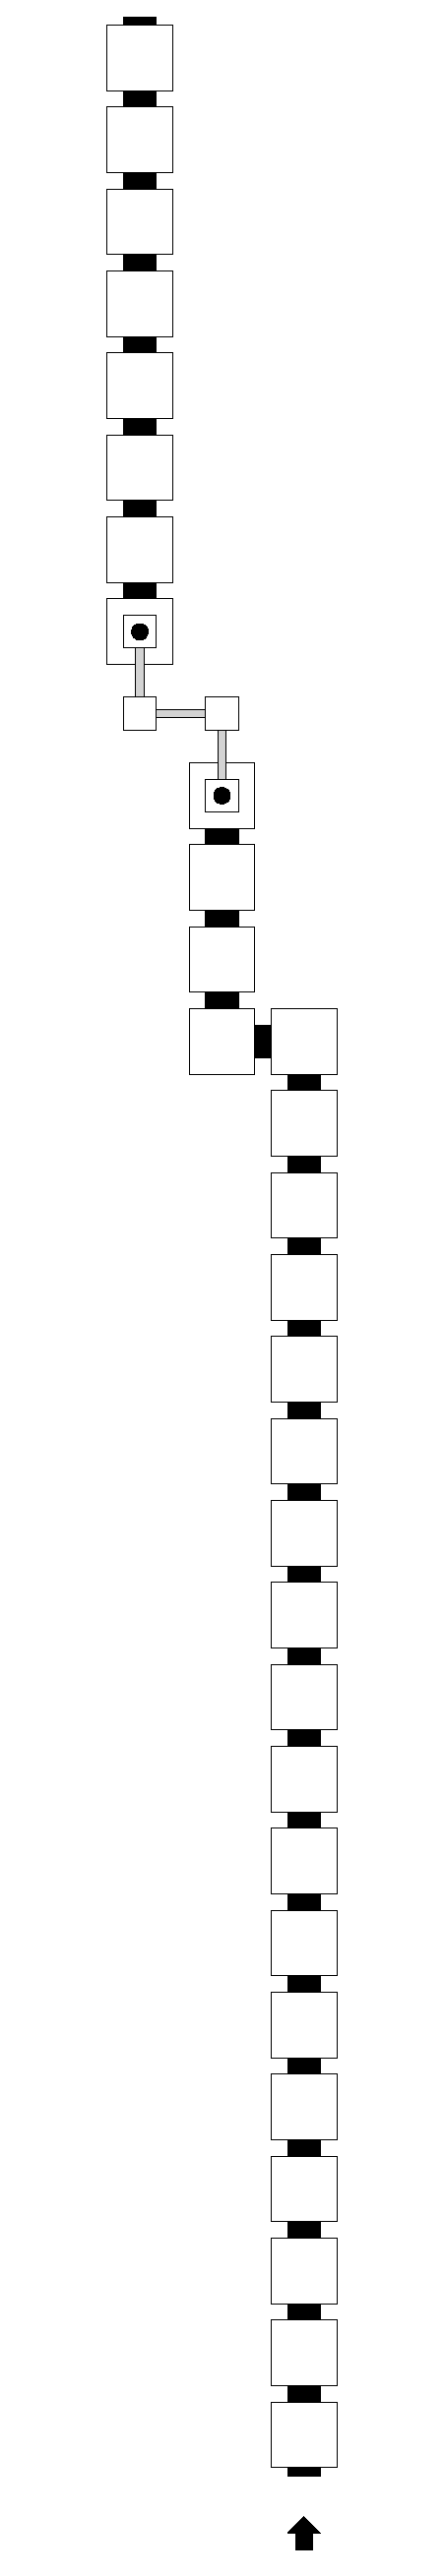
\includegraphics[width=0.45in]{warping_pre_warp_general}}}%
        ~
        \subcaptionbox{
            Digit 1 - general\\overview.
            The black tiles in this figure correspond to the gadget shown in subfigure~\subref{fig:pre_warp_general}.
            \label{fig:pre_warp_1_op_overview}
        }{\makebox[0.24\textwidth][c]{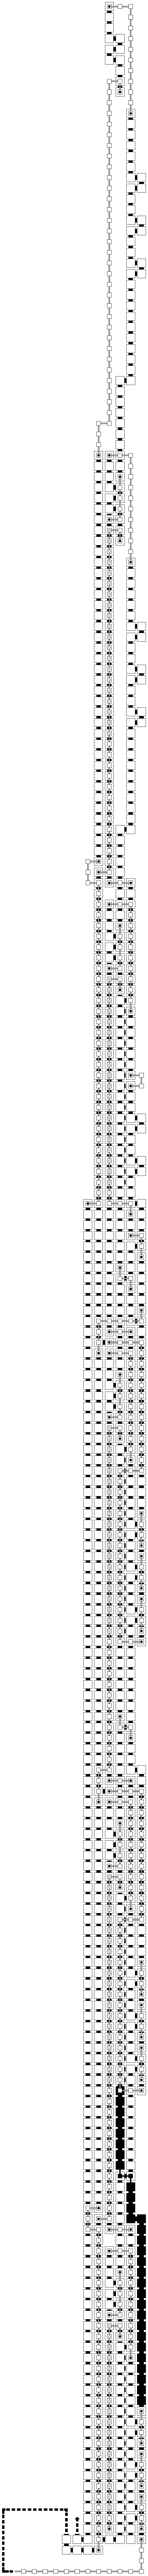
\includegraphics[width=0.45in]{overviews/general/pre_warp_1_op}}}%
        ~
        \subcaptionbox{
            Digit 2 - general\\overview.
            The black tiles in this figure correspond to the gadget shown in subfigure~\subref{fig:pre_warp_general}.
            \label{fig:pre_warp_2_op_overview}
        }{\makebox[0.24\textwidth][c]{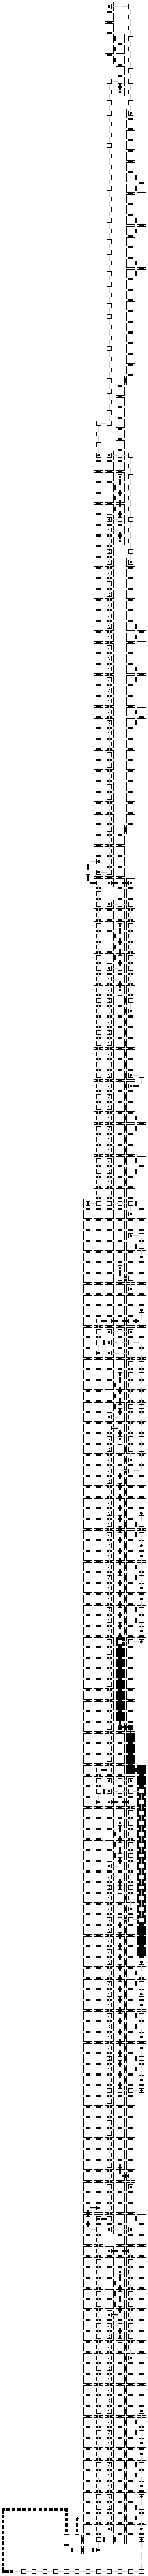
\includegraphics[width=0.45in]{overviews/general/pre_warp_2_op}}}%
        ~
        \subcaptionbox{
            Digit 3 - general\\overview.
            The black tiles in this figure correspond to the gadget shown in subfigure~\subref{fig:pre_warp_general}.
            \label{fig:pre_warp_3_op_overview}
        }{\makebox[0.24\textwidth][c]{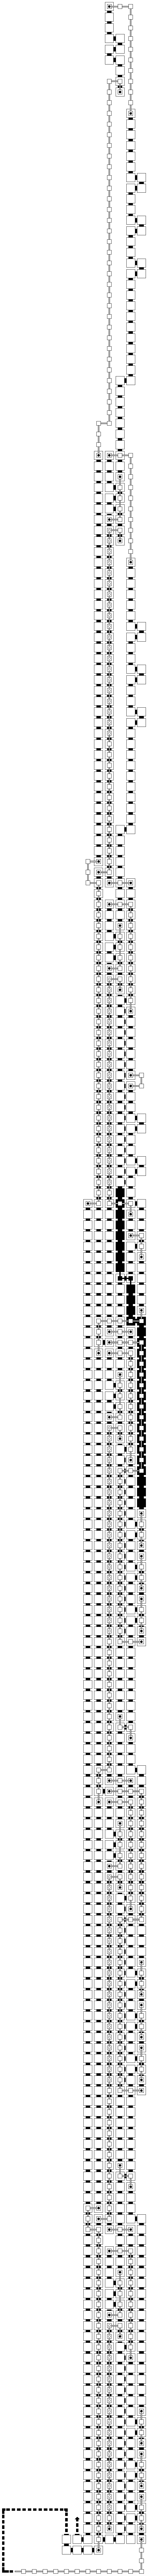
\includegraphics[width=0.45in]{overviews/general/pre_warp_3_op}}}%
        ~
    \end{figure}
    \begin{figure}[H]\ContinuedFloat
        \centering
        \subcaptionbox{
            Digit 1 - case 1. There are 31 tiles in this gadget.
            \label{fig:pre_warp_1_op_msr_msd}
        }{\makebox[0.24\textwidth][c]{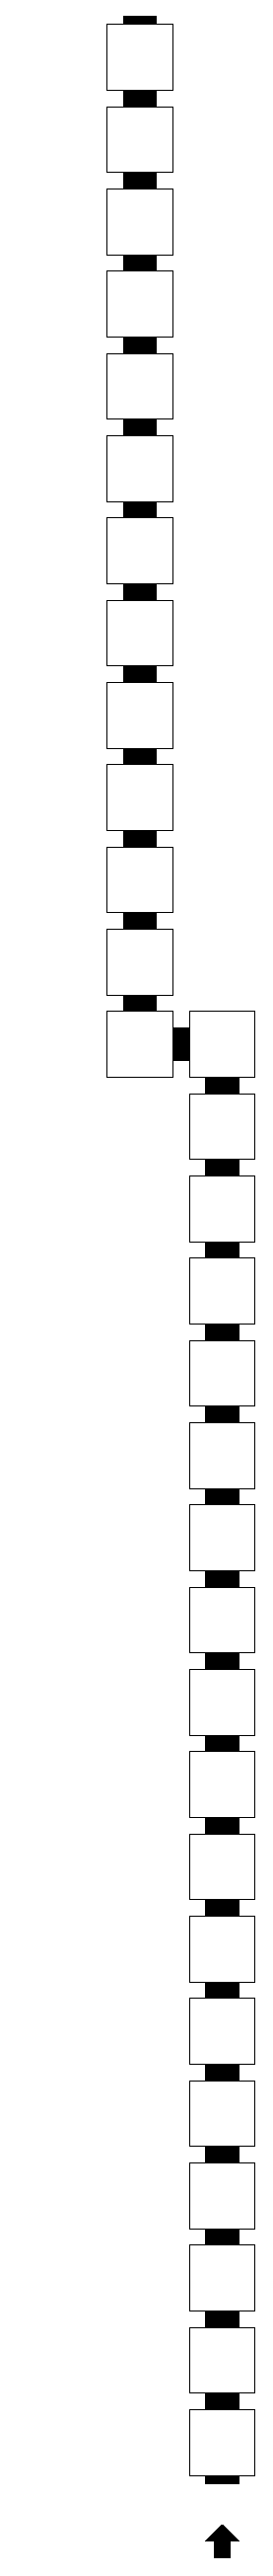
\includegraphics[width=0.45in]{warping_pre_warp_case1_digit1_msr}}}%
        ~
        \subcaptionbox{
            Digit 1 - case 1 overview.
            The black tiles in this figure correspond to the gadget shown in subfigure~\subref{fig:pre_warp_1_op_msr_msd}.
            \label{fig:pre_warp_1_op_msr_msd_overview}
        }{\makebox[0.24\textwidth][c]{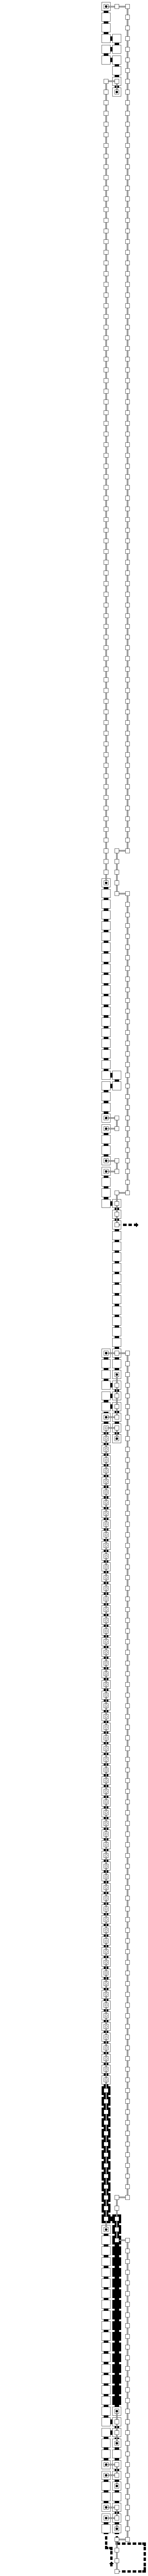
\includegraphics[width=0.45in]{overviews/case1/pre_warp_1_op_msr_msd}}}%
        ~
        \subcaptionbox{
            Digit 1 - case 2. There are 34 tiles in this gadget.
            \label{fig:pre_warp_1_op_msr}
        }{\makebox[0.24\textwidth][c]{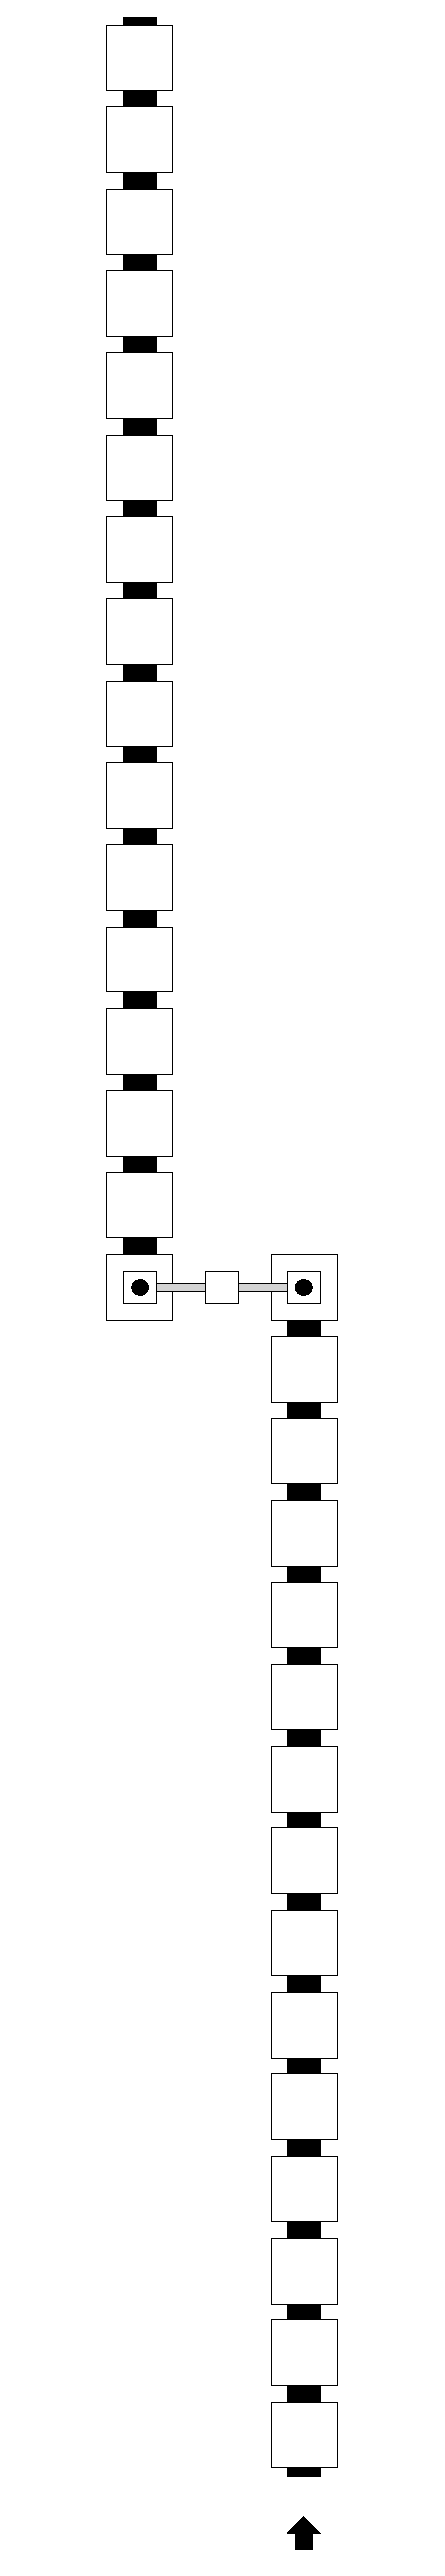
\includegraphics[width=0.45in]{warping_pre_warp_case2_digit1_msr}}}%
        ~
        \subcaptionbox{
            Digit 1 - case 2 overview.
            The black tiles in this figure correspond to the gadget shown in subfigure~\subref{fig:pre_warp_1_op_msr}.
            \label{fig:pre_warp_1_op_msr_overview}
        }{\makebox[0.24\textwidth][c]{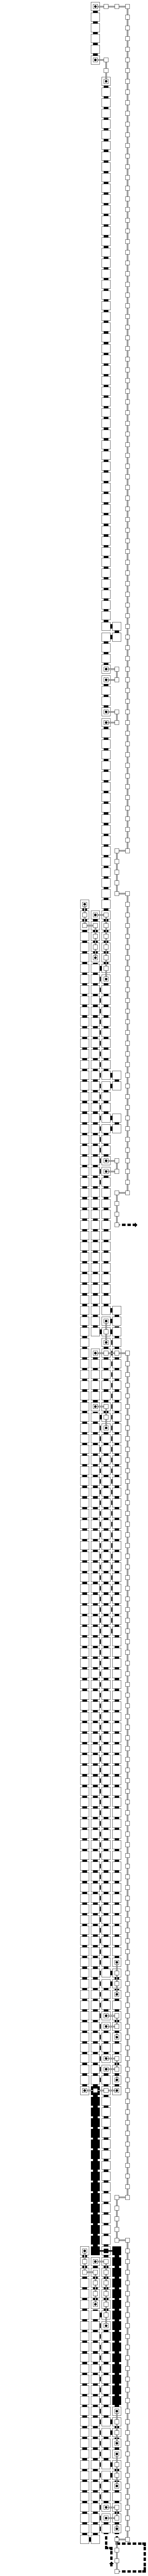
\includegraphics[width=0.45in]{overviews/case2/pre_warp_1_op_msr}}}%
        ~
    \end{figure}
    \begin{figure}[H]\ContinuedFloat
        \centering
        \subcaptionbox{
            Digit 2 - case 2. There are 30 tiles in this gadget.
            \label{fig:pre_warp_2_op_msr_msd}
        }{\makebox[0.32\textwidth][c]{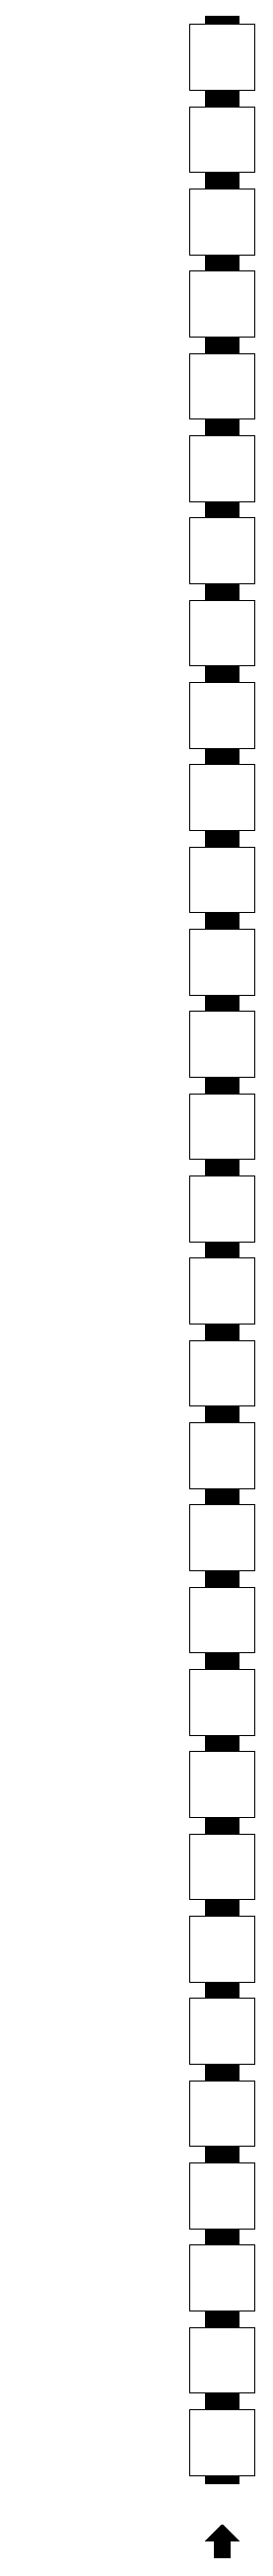
\includegraphics[width=0.45in]{warping_pre_warp_case2_digit2_msr}}}%
        ~
        \subcaptionbox{
            Digit 2 - case 2 overview.
            The black tiles in this figure correspond to the gadget shown in subfigure~\subref{fig:pre_warp_2_op_msr_msd}.
            \label{fig:pre_warp_2_op_msr_msd_overview}
        }{\makebox[0.32\textwidth][c]{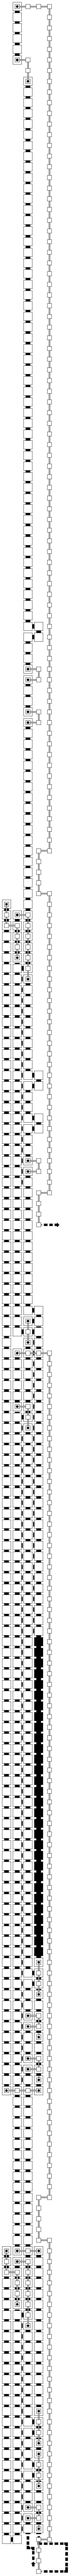
\includegraphics[width=0.45in]{overviews/case2/pre_warp_2_op_msr_msd}}}%
        ~
        \subcaptionbox{
            Digit 3 - case 3 overview.
            The black tiles in this figure correspond to the gadget shown in subfigure~\subref{fig:pre_warp_general}.
            \label{fig:pre_warp_3_op_msr_msd_overview}
        }{\makebox[0.32\textwidth][c]{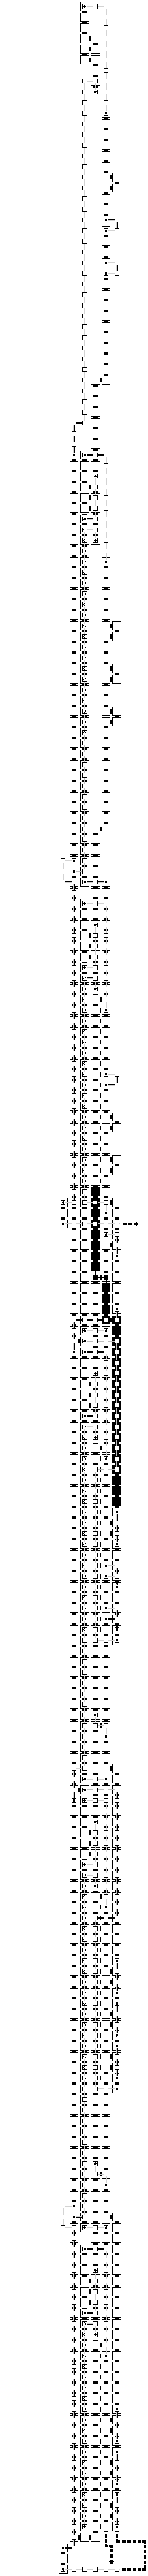
\includegraphics[width=0.45in]{overviews/case3/pre_warp_3_op_msr_msd}}}%
        ~
        \caption{\label{fig:pre_warp_gadgets} The {\prewarp} gadgets.}
    \end{figure}


    \item {\firstwarp}:
    \\
    The idea of the {\firstwarp} gadget is to transport the information read by the {\cread} gadgets, usually across a large distance.
    %
    We do this using a single special tile that has three glues.
    %
    Both the north and south glues have the same labels, allowing this tile to assemble into a line indefinitely.
    %
    The third glue is the special glue; this glue can be either on the east or west side of the tile, and has the output label.
    %
    This unique glue will at some point later in the assembly, in a spot determined by earlier pieces of the assembly, no longer be blocked from the direction of it special glue.
    %
    When this occurs, it can finally attach to the {\warpbridge} gadget (except in a few special cases where the {\warpbridge} gadget is skipped).
    %
    This process signifies the ``waking up'' of the {\firstwarp} gadgets.
    %
    When this gadget wakes up, it must also be blocked in the north direction.
    %
    By blocking the north glue, the line stops, which prevents a truly infinite line from assembling.
    %
    The earlier pieces of the assembly that guarentee this process to work are known as the {\dtop} gadgets.
    %

    For each $i = 1, 2, 3$, $u \in \{0, 1\}^l$, and each $\inc \in \ops$:
    \begin{itemize}
        \item Create
        $\begin{aligned}[t]
            \firstwarp(& \left\langle {\tt FirstWarp},  i, u, \inc \right\rangle,\\  % South
                       & \left\langle {\tt FirstWarp},  i, u, \inc \right\rangle,\\  % North
                       & \left\langle {\tt WarpBridge}, i, u, \inc \right\rangle \;) % East
        \end{aligned}$\\ from the single tile gadget, shown in Figure~\ref{fig:first_warp_1_op_overview}
                         if $i = 1$ or Figure~\ref{fig:first_warp_2_op_overview} if $i = 2$, otherwise from
                         Figure~\ref{fig:first_warp_3_op_overview} if $i = 3$.
        \vspace{.5cm}
        \item Create
        $\begin{aligned}[t]
            \firstwarp(& \left\langle {\tt FirstWarp}, 1, u, \inc, {\tt msr} \right\rangle, \\ % South
                       & \left\langle {\tt FirstWarp}, 1, u, \inc, {\tt msr} \right\rangle, \\ % North
                       & \left\langle {\tt PostWarp},  1, u, \inc, {\tt msr} \right\rangle \;) % East
        \end{aligned}$\\ from the single tile gadget shown in Figure~\ref{fig:first_warp_1_op_msr_overview}.
        \vspace{.5cm}
        \item Create
        $\begin{aligned}[t]
            \firstwarp(& \left\langle {\tt FirstWarp}, 1, u, \inc, {\tt msr}, {\tt msd} \right\rangle, \\ % South
                       & \left\langle {\tt FirstWarp}, 1, u, \inc, {\tt msr}, {\tt msd} \right\rangle, \\ % North
                       & \left\langle {\tt PostWarp},  1, u, \inc, {\tt msr}, {\tt msd} \right\rangle \;) % Up
        \end{aligned}$\\ from the single tile gadget shown in Figure~\ref{fig:first_warp_1_op_msr_msd_overview}.
        \vspace{.5cm}
        \item Create
        $\begin{aligned}[t]
            \firstwarp(& \left\langle {\tt FirstWarp},  2, u, \inc, {\tt msr}, {\tt msd} \right\rangle, \\ % South
                       & \left\langle {\tt FirstWarp},  2, u, \inc, {\tt msr}, {\tt msd} \right\rangle, \\ % North
                       & \left\langle {\tt WarpBridge}, 2, u, \inc, {\tt msr}, {\tt msd} \right\rangle \;) % West
        \end{aligned}$\\ from the single tile gadget shown in Figure~\ref{fig:first_warp_2_op_msr_msd_overview}.
        \vspace{.5cm}
        \item Create
        $\begin{aligned}[t]
            \firstwarp(& \left\langle {\tt FirstWarp},  3, u, \inc, {\tt msr}, {\tt msd} \right\rangle,\\  % South
                       & \left\langle {\tt FirstWarp},  3, u, \inc, {\tt msr}, {\tt msd} \right\rangle,\\  % North
                       & \left\langle {\tt WarpBridge}, 3, u, \inc, {\tt msr}, {\tt msd} \right\rangle \;) % East
        \end{aligned}$\\ from the single tile gadget shown in Figure~\ref{fig:first_warp_3_op_msr_msd_overview}.
        \vspace{.5cm}
    \end{itemize}
    \vspace{.5cm}

    In this step, for digits 1-3 in the general case,
    %
    $9 \cdot 2^l =$
    %
    $9 \cdot 2^{\ceil*{{\log m}} + 2} =$
    %
    $36 \cdot 2^{\ceil*{\log m}} \leq$
    %
    $72 \cdot 2^{\log m} = \bigom$ tiles were created.
    %

    For digit 1 in case 1,
    %
    $3 \cdot 2^l =$
    %
    $3 \cdot 2^{\ceil*{{\log m}} + 2} =$
    %
    $12 \cdot 2^{\ceil*{\log m}} \leq$
    %
    $24 \cdot 2^{\log m} = \bigom$ tiles were created.
    %

    For digit 1 in case 2,
    %
    $3 \cdot 2^l =$
    %
    $3 \cdot 2^{\ceil*{{\log m}} + 2} =$
    %
    $12 \cdot 2^{\ceil*{\log m}} \leq$
    %
    $24 \cdot 2^{\log m} = \bigom$ tiles were created.
    %

    For digit 2 in case 2,
    %
    $3 \cdot 2^l =$
    %
    $3 \cdot 2^{\ceil*{{\log m}} + 2} =$
    %
    $12 \cdot 2^{\ceil*{\log m}} \leq$
    %
    $24 \cdot 2^{\log m} = \bigom$ tiles were created.
    %

    For digit 3 in case 3,
    %
    $3 \cdot 2^l =$
    %
    $3 \cdot 2^{\ceil*{{\log m}} + 2} =$
    %
    $12 \cdot 2^{\ceil*{\log m}} \leq$
    %
    $24 \cdot 2^{\log m} = \bigom$ tiles were created.
    %

    \begin{figure}[H]
        \centering
        \subcaptionbox{
            Digit 1 - general\\ overview.
            \label{fig:first_warp_1_op_overview}
        }{\makebox[0.24\textwidth][c]{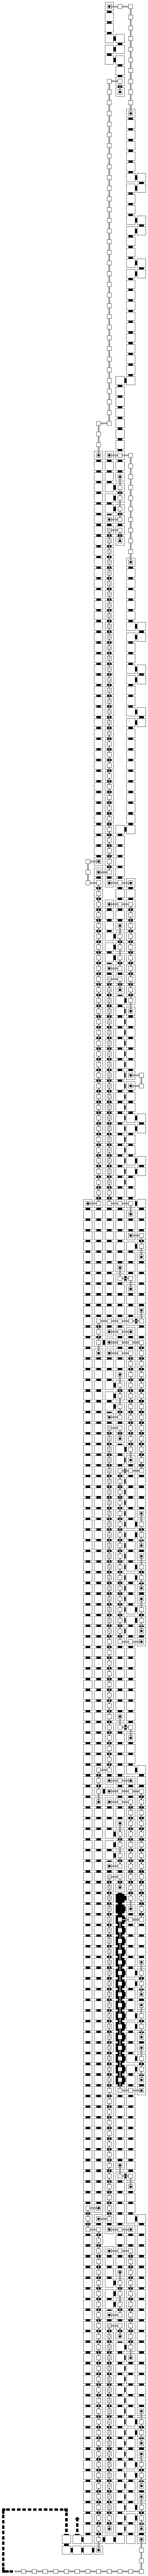
\includegraphics[width=0.45in]{overviews/general/first_warp_1_op}}}%
        ~
        \subcaptionbox{
            Digit 2 - general\\ overview.
            \label{fig:first_warp_2_op_overview}
        }{\makebox[0.24\textwidth][c]{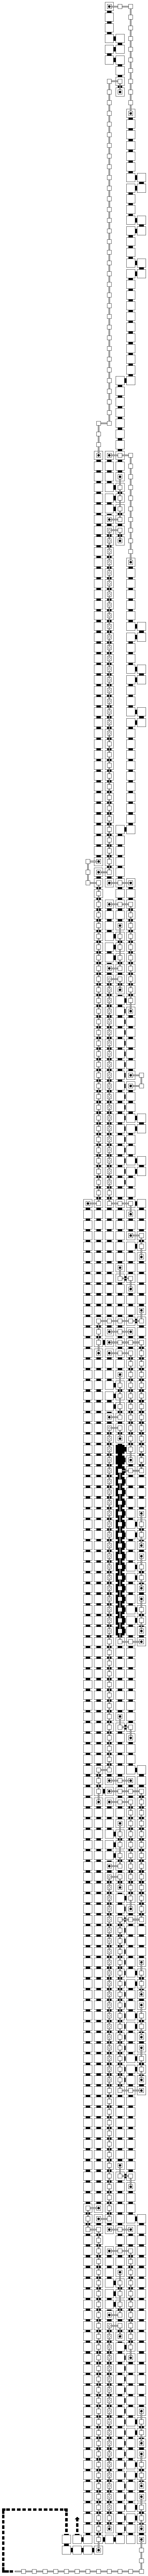
\includegraphics[width=0.45in]{overviews/general/first_warp_2_op}}}%
        ~
        \subcaptionbox{
            Digit 3 - general\\ overview.
            \label{fig:first_warp_3_op_overview}
        }{\makebox[0.24\textwidth][c]{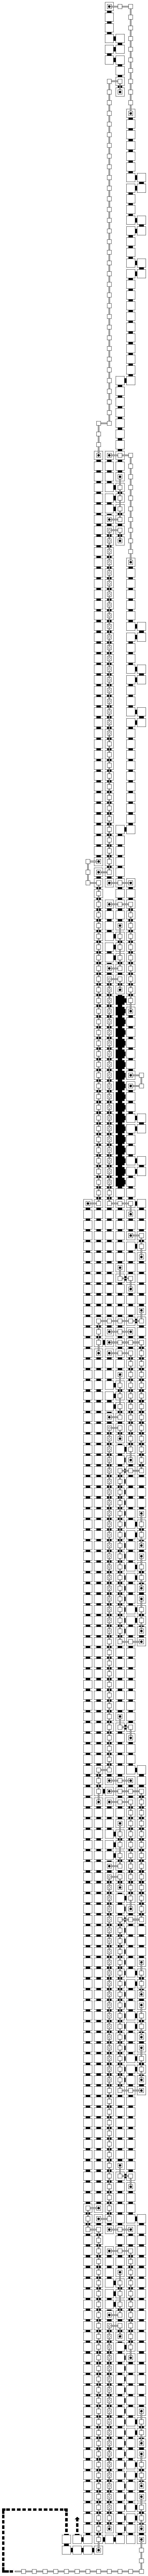
\includegraphics[width=0.45in]{overviews/general/first_warp_3_op}}}%
        ~
        \subcaptionbox{
            Digit 3 - general (seed) overview.
            \label{fig:first_warp_3_seed_op_overview}
        }{\makebox[0.24\textwidth][c]{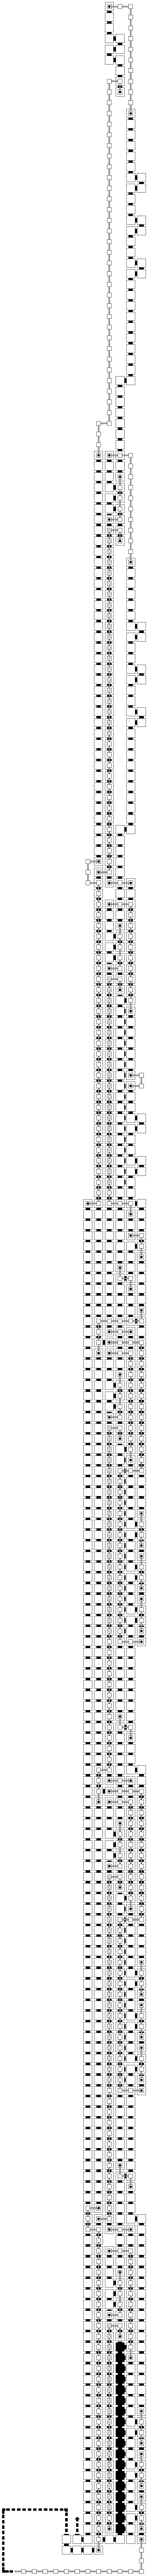
\includegraphics[width=0.45in]{overviews/general/first_warp_3_seed_op}}}%
        ~
    \end{figure}
    \begin{figure}[H]\ContinuedFloat
        \centering
        \subcaptionbox{
            Digit 1 - case 1 overview.
            \label{fig:first_warp_1_op_msr_msd_overview}
        }{\makebox[0.24\textwidth][c]{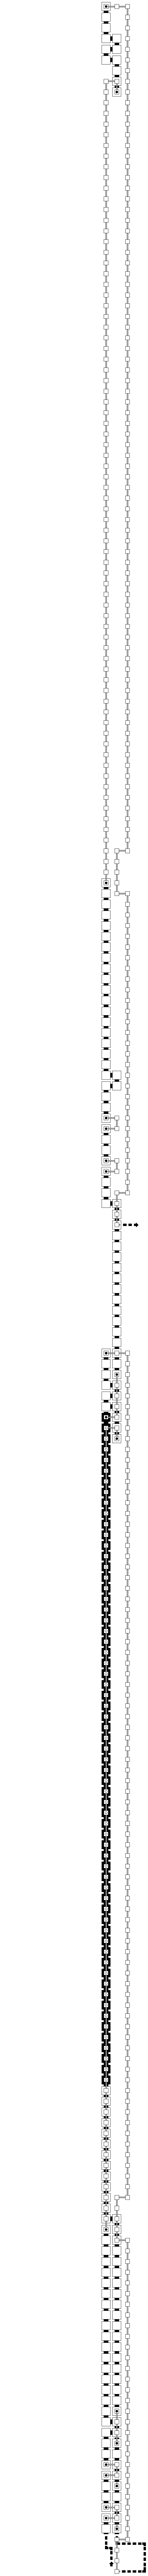
\includegraphics[width=0.45in]{overviews/case1/first_warp_1_op_msr_msd}}}%
        ~
        \subcaptionbox{
            Digit 1 - case 2 overview.
            \label{fig:first_warp_1_op_msr_overview}
        }{\makebox[0.24\textwidth][c]{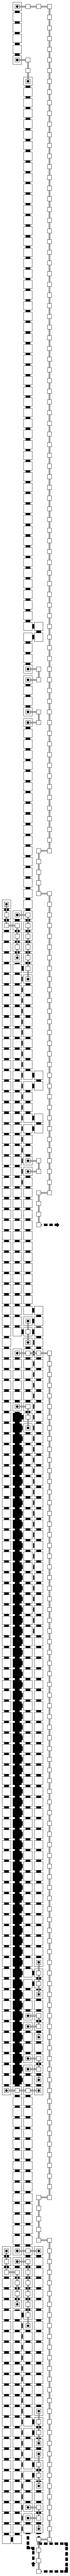
\includegraphics[width=0.45in]{overviews/case2/first_warp_1_op_msr}}}%
        ~
        \subcaptionbox{
            Digit 2 - case 2 overview.
            \label{fig:first_warp_2_op_msr_msd_overview}
        }{\makebox[0.24\textwidth][c]{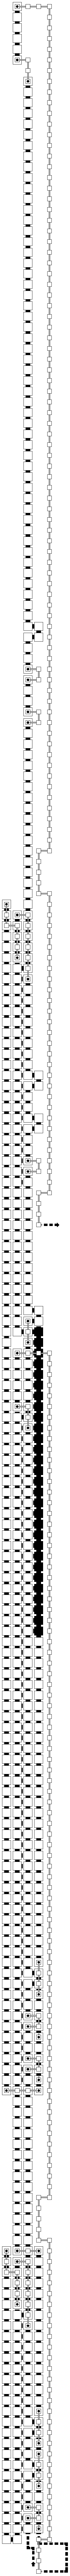
\includegraphics[width=0.45in]{overviews/case2/first_warp_2_op_msr_msd}}}%
        ~
        \subcaptionbox{
            Digit 3 - case 3 overview.
            \label{fig:first_warp_3_op_msr_msd_overview}
        }{\makebox[0.24\textwidth][c]{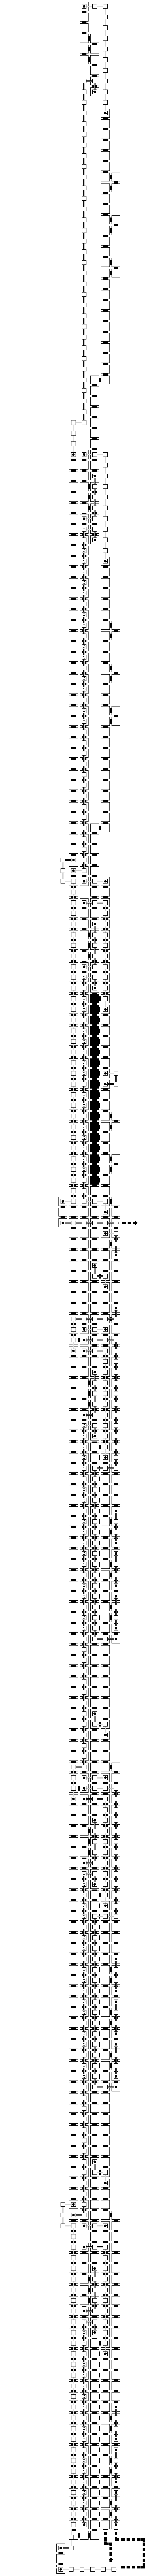
\includegraphics[width=0.45in]{overviews/case3/first_warp_3_op_msr_msd}}}%
        ~
        \caption{\label{fig:first_warp_gadgets_overviews} The {\firstwarp} gadget overviews.}
    \end{figure}


    \item {\warpbridge}:\\
    %
    The idea of the {\warpbridge} gadget is to assemble after the {\firstwarp} gadget makes it to its final destination.
    %
    Its objective is to assemble a path from the end of the {\firstwarp} gadgets to the start of the {\secondwarp} gadgets.
    %
    For digit 1 in cases 1 and 2, the {\warpbridge} is omitted from the {\warpunit}.
    %

    For each $i = 1,2,3, u \in \{0, 1\}^l$, and each $\inc \in \ops$:
    \begin{itemize}

        \item Create
        $\begin{aligned}[t]
            \warpbridge(& \left\langle {\tt WarpBridge}, i, u, \inc \right\rangle,
                          \left\langle {\tt SecondWarp}, i, u, \inc \right\rangle \;)
        \end{aligned}$ \\ from the general gadget in Figure~\ref{fig:warp_bridge_general}.
        \vspace{.5cm}

        \item Create
        $\begin{aligned}[t]
            \warpbridge(& \left\langle {\tt WarpBridge}, 2, u, \inc, {\tt msr}, {\tt msd} \right\rangle,
                          \left\langle {\tt SecondWarp}, 2, u, \inc, {\tt msr}, {\tt msd} \right\rangle \;)
        \end{aligned}$ \\ from the general gadget in Figure~\ref{fig:warp_bridge_2_op_msr_msd}.
        \vspace{.5cm}

        \item Create
        $\begin{aligned}[t]
            \warpbridge(& \left\langle {\tt WarpBridge}, 3, u, \inc, {\tt msr}, {\tt msd} \right\rangle,
                          \left\langle {\tt SecondWarp}, 3, u, \inc, {\tt msr}, {\tt msd} \right\rangle \;)
        \end{aligned}$ \\ from the general gadget in Figure~\ref{fig:warp_bridge_general}.
        \vspace{.5cm}
    \end{itemize}

    In this step, for digits 1-3 in the general case,
    %
    $9 \cdot 2^l \cdot 29 =$
    %
    $261 \cdot 2^l =$
    %
    $261 \cdot 2^{\ceil*{{\log m}} + 2} =$
    %
    $1044 \cdot 2^{\ceil*{\log m}} \leq$
    %
    $2088 \cdot 2^{\log m} = \bigom$ tiles were created.
    %

    For digit 2 in case 2,
    %
    $3 \cdot 2^l \cdot 15 =$
    %
    $45 \cdot 2^l =$
    %
    $45 \cdot 2^{\ceil*{{\log m}} + 2} =$
    %
    $180 \cdot 2^{\ceil*{\log m}} \leq$
    %
    $360 \cdot 2^{\log m} = \bigom$ tiles were created.
    %

    For digit 3 in case 3,
    %
    $3 \cdot 2^l \cdot 29 =$
    %
    $87 \cdot 2^l =$
    %
    $87 \cdot 2^{\ceil*{{\log m}} + 2} =$
    %
    $348 \cdot 2^{\ceil*{\log m}} \leq$
    %
    $696 \cdot 2^{\log m} = \bigom$ tiles were created.
    %

    \begin{figure}[H]
        \centering
        \subcaptionbox{
            Digits 1, 2, \& 3 general, digit 3 - case 3. There are 29 tiles in this gadget.
            \label{fig:warp_bridge_general}
        }{\makebox[0.24\textwidth][c]{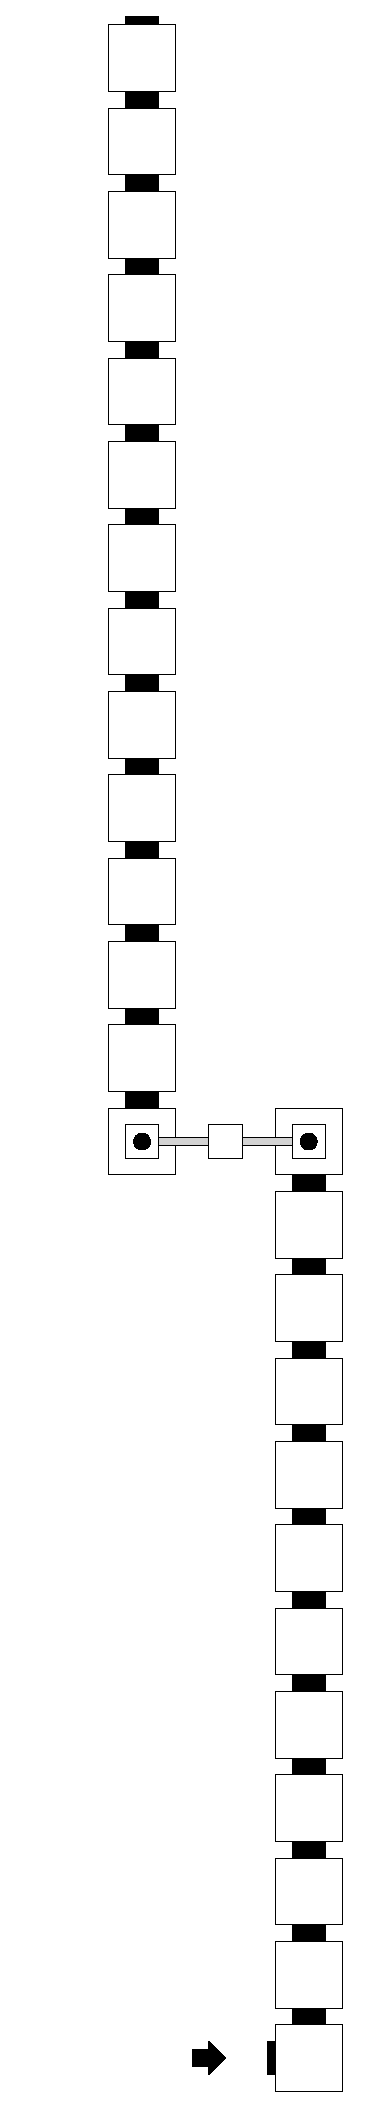
\includegraphics[width=0.45in]{warping_warp_bridge_general}}}%
        ~
        \subcaptionbox{
            Digit 1 - general\\ overview.
            The black tiles in this figure correspond to the gadget shown in subfigure~\subref{fig:warp_bridge_general}.
            \label{fig:warp_bridge_1_op_overview}
        }{\makebox[0.24\textwidth][c]{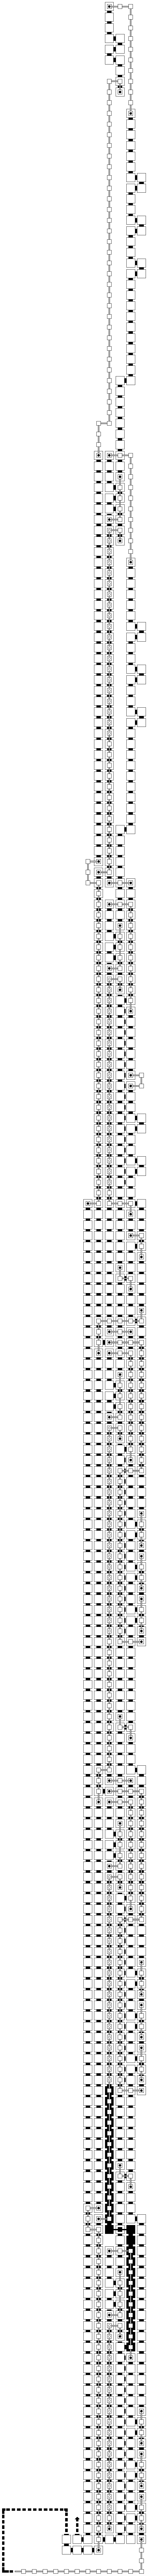
\includegraphics[width=0.45in]{overviews/general/warp_bridge_1_op}}}%
        ~
        \subcaptionbox{
            Digit 2 - general\\ overview.
            The black tiles in this figure correspond to the gadget shown in subfigure~\subref{fig:warp_bridge_general}.
            \label{fig:warp_bridge_2_op_overview}
        }{\makebox[0.24\textwidth][c]{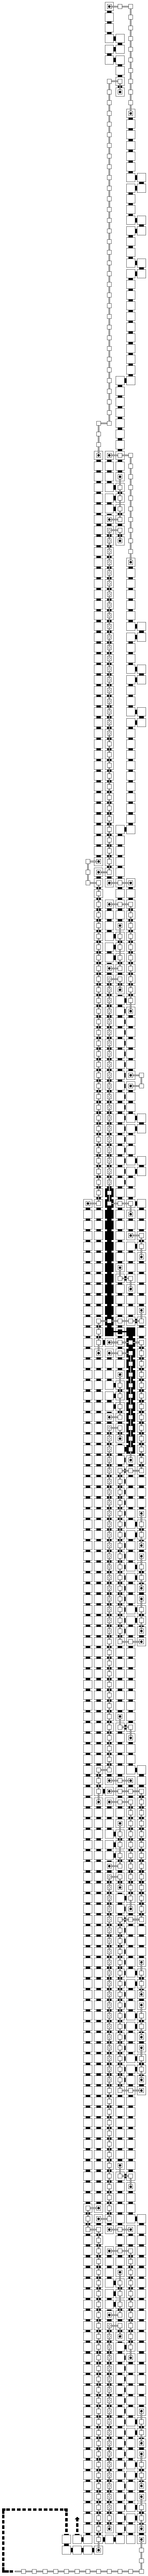
\includegraphics[width=0.45in]{overviews/general/warp_bridge_2_op}}}%
        ~
        \subcaptionbox{
            Digit 2 - general (seed) overview.
            The black tiles in this figure correspond to the gadget shown in subfigure~\subref{fig:warp_bridge_general}.
            \label{fig:warp_bridge_2_seed_op_overview}
        }{\makebox[0.24\textwidth][c]{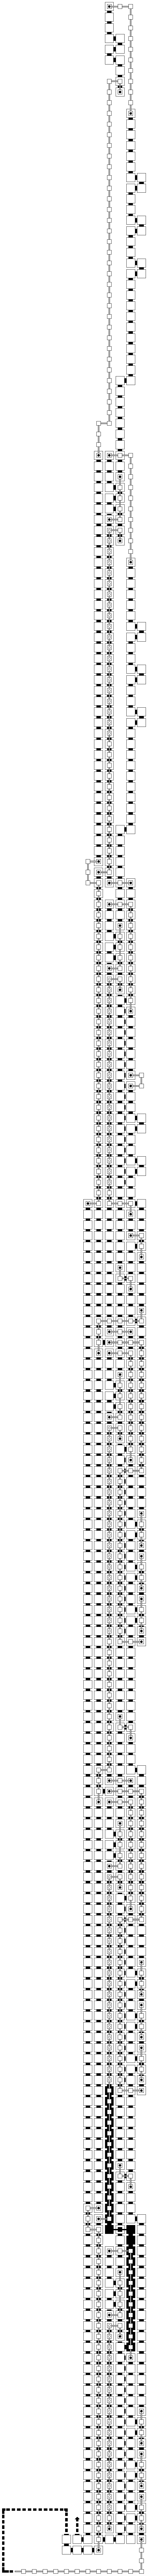
\includegraphics[width=0.45in]{overviews/general/warp_bridge_2_seed_op}}}%
        ~
    \end{figure}
    \begin{figure}[H]\ContinuedFloat
        \centering
        \subcaptionbox{
            Digit 3 - general\\ overview.
            The black tiles in this figure correspond to the gadget shown in subfigure~\subref{fig:warp_bridge_general}.
            \label{fig:warp_bridge_3_op_overview}
        }{\makebox[0.24\textwidth][c]{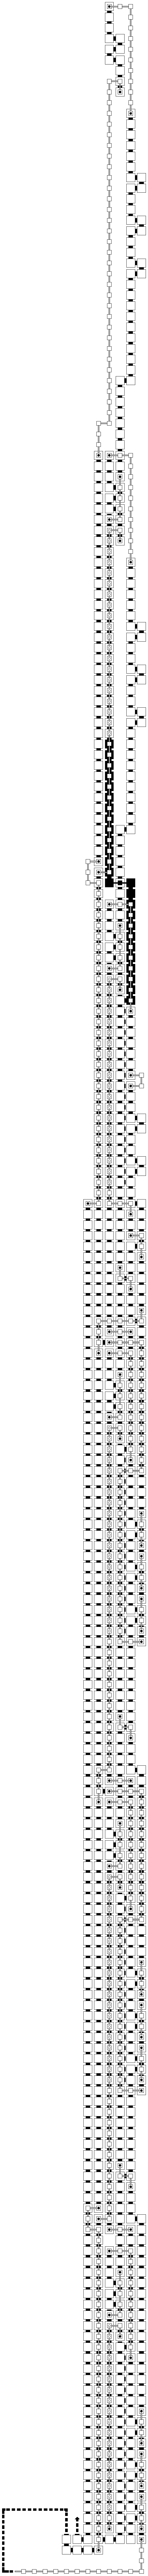
\includegraphics[width=0.45in]{overviews/general/warp_bridge_3_op}}}%
        ~
        \subcaptionbox{
            Digit 3 - general (seed) overview.
            The black tiles in this figure correspond to the gadget shown in subfigure~\subref{fig:warp_bridge_general}.
            \label{fig:warp_bridge_3_seed_op_overview}
        }{\makebox[0.24\textwidth][c]{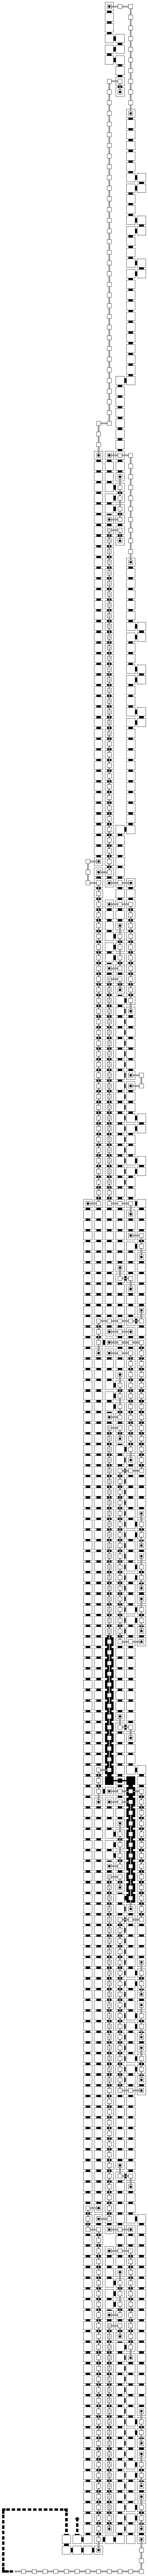
\includegraphics[width=0.45in]{overviews/general/warp_bridge_3_seed_op}}}%
        ~
        \subcaptionbox{
            Digit 2 - case 2. There are 15 tiles in this gadget.
            \label{fig:warp_bridge_2_op_msr_msd}
        }{\makebox[0.24\textwidth][c]{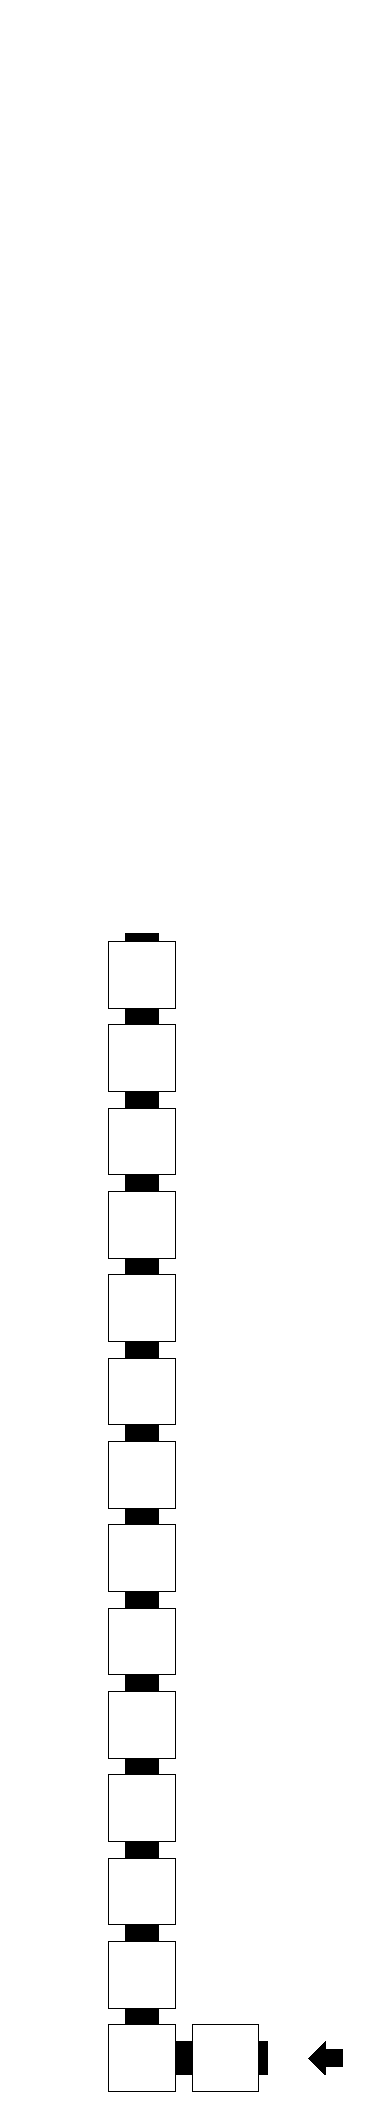
\includegraphics[width=0.45in]{warping_warp_bridge_case2_digit2_msr}}}%
        ~
        \subcaptionbox{
            Digit 2 - case 2 overview.
            The black tiles in this figure correspond to the gadget shown in subfigure~\subref{fig:warp_bridge_2_op_msr_msd}.
            \label{fig:warp_bridge_2_op_msr_msd_overview}
        }{\makebox[0.24\textwidth][c]{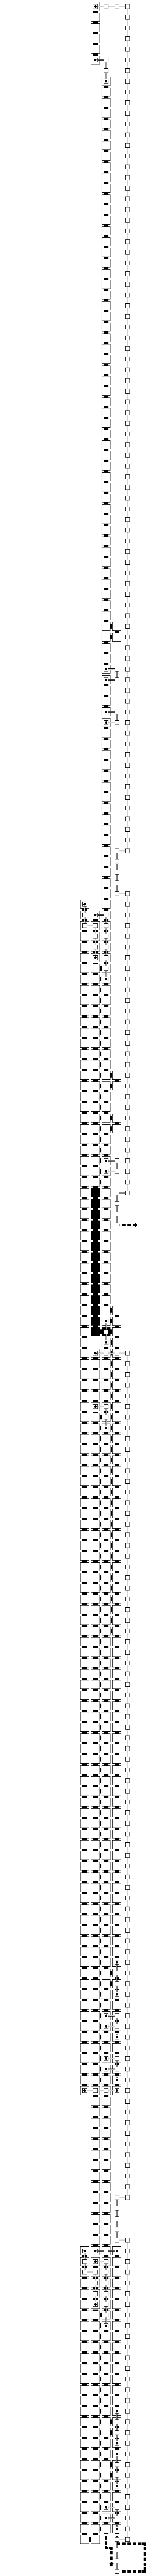
\includegraphics[width=0.45in]{overviews/case2/warp_bridge_2_op_msr_msd}}}%
        ~
    \end{figure}
    \begin{figure}[H]\ContinuedFloat
        \centering
        \subcaptionbox{
            Digit 3 - case 3 overview.
            The black tiles in this figure correspond to the gadget shown in subfigure~\subref{fig:warp_bridge_general}.
            \label{fig:warp_bridge_3_op_msr_msd_overview}
        }{\makebox[0.49\textwidth][c]{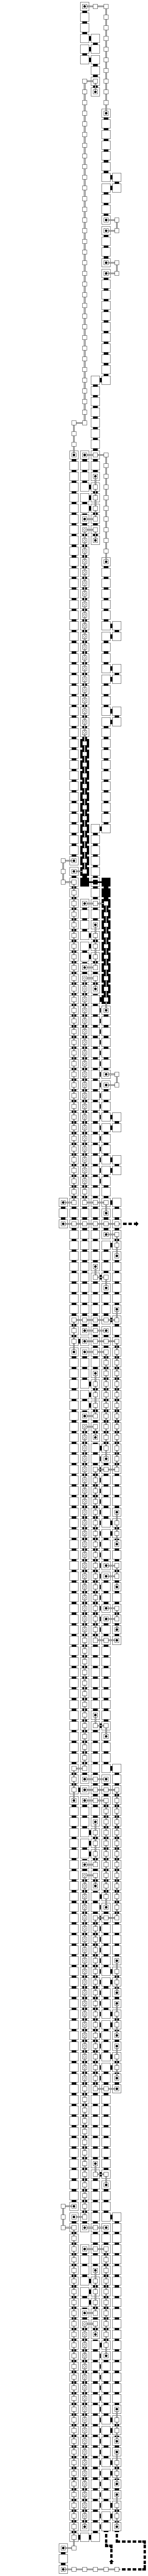
\includegraphics[width=0.45in]{overviews/case3/warp_bridge_3_op_msr_msd}}}%
        ~
        \subcaptionbox{
            Digit 3 - case 3 (seed) overview.
            The black tiles in this figure correspond to the gadget shown in subfigure~\subref{fig:warp_bridge_general}.
            \label{fig:warp_bridge_3_seed_op_msr_msd_overview}
        }{\makebox[0.49\textwidth][c]{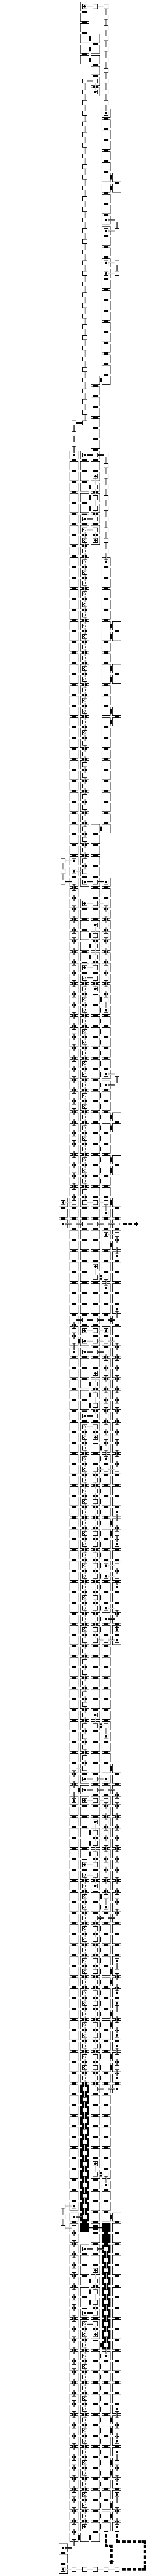
\includegraphics[width=0.45in]{overviews/case3/warp_bridge_3_seed_op_msr_msd}}}%
        ~
        \caption{\label{fig:warp_bridge_gadgets_overviews} The {\warpbridge} gadgets.}
    \end{figure}

    \item {\secondwarp}: \\
    %
    Similar to the {\firstwarp} gadget, the idea of this gadget is also transport the information read by the {\cread} gadgets across a large distance.
    %
    We do this using a single special tile that has three glues.
    %
    Both the north and south glues have the same labels, allowing this tile to assemble into a line indefinitely.
    %
    The third glue is also the special glue; this glue can be either on the east or up side of the tile, and has the output label.
    %
    This unique glue will at some point later in the assembly, in a spot determined by earlier pieces of the assembly, no longer be blocked from the direction of it special glue.
    %
    When this occurs, it can finally attach to the {\postwarp} gadget.
    %
    This process signifies the ``waking up'' of the {\secondwarp} gadgets.
    %
    When this gadget wakes up, it must also be blocked in the north direction.
    %
    By blocking the north glue, the line stops, which prevents a truly infinite line from assembling.
    %
    The earlier pieces of the assembly that guarentee this process to work are known as the {\dtop} gadgets.
    %

    For each $i = 1,2,3, u \in \{0, 1\}^l$, and each $\inc \in \ops$:
    \begin{itemize}
        \item Create
        $\begin{aligned}[t]
            \secondwarp(& \left\langle {\tt SecondWarp}, i, u, \inc \right\rangle,     % South
                          \left\langle {\tt SecondWarp}, i, u, \inc \right\rangle,     % North
                          \left\langle {\tt PostWarp},   i, u, \inc \right\rangle \;)  % Up
        \end{aligned}$\\ from the single tile gadget, shown in Figure~\ref{fig:second_warp_1_op_overview}
                         if $i = 1$ or Figure~\ref{fig:second_warp_2_op_overview} if $i = 2$, otherwise from
                         Figure~\ref{fig:second_warp_3_op_overview} if $i = 3$.
        \vspace{0.5cm}

        \item Create
        $\begin{aligned}[t]
            \secondwarp(& \left\langle {\tt SecondWarp}, 2, u, \inc, {\tt msr}, {\tt msd} \right\rangle, \\ % South
                        & \left\langle {\tt SecondWarp}, 2, u, \inc, {\tt msr}, {\tt msd} \right\rangle, \\ % North
                        & \left\langle {\tt PostWarp},   2, u, \inc, {\tt msr}, {\tt msd} \right\rangle \;) % East
        \end{aligned}$\\ from the single tile gadget shown in Figure~\ref{fig:second_warp_2_op_msr_msd_overview}.
        \vspace{0.5cm}

        \item Create
        $\begin{aligned}[t]
            \secondwarp(& \left\langle {\tt SecondWarp}, 3, u, \inc, {\tt msr}, {\tt msd} \right\rangle, \\ % South
                        & \left\langle {\tt SecondWarp}, 3, u, \inc, {\tt msr}, {\tt msd} \right\rangle, \\ % North
                        & \left\langle {\tt PostWarp},   3, u, \inc, {\tt msr}, {\tt msd} \right\rangle \;) % Up
        \end{aligned}$\\ from the single tile gadget shown in Figure~\ref{fig:second_warp_3_op_msr_msd_overview}.
    \end{itemize}

    In this step, for digits 1-3 in the general case,
    %
    $9 \cdot 2^l =$
    %
    $9 \cdot 2^{\ceil*{{\log m}} + 2} =$
    %
    $36 \cdot 2^{\ceil*{\log m}} \leq$
    %
    $72 \cdot 2^{\log m} = \bigom$ tiles were created.
    %

    For digit 2 in case 2,
    %
    $3 \cdot 2^l =$
    %
    $3 \cdot 2^{\ceil*{{\log m}} + 2} =$
    %
    $12 \cdot 2^{\ceil*{\log m}} \leq$
    %
    $24 \cdot 2^{\log m} = \bigom$ tiles were created.
    %

    For digit 3 in case 3,
    %
    $3 \cdot 2^l =$
    %
    $3 \cdot 2^{\ceil*{{\log m}} + 2} =$
    %
    $12 \cdot 2^{\ceil*{\log m}} \leq$
    %
    $24 \cdot 2^{\log m} = \bigom$ tiles were created.
    %

    \begin{figure}[H]
        \centering
        \subcaptionbox{
            Digit 1 - general\\ overview.
            \label{fig:second_warp_1_op_overview}
        }{\makebox[0.24\textwidth][c]{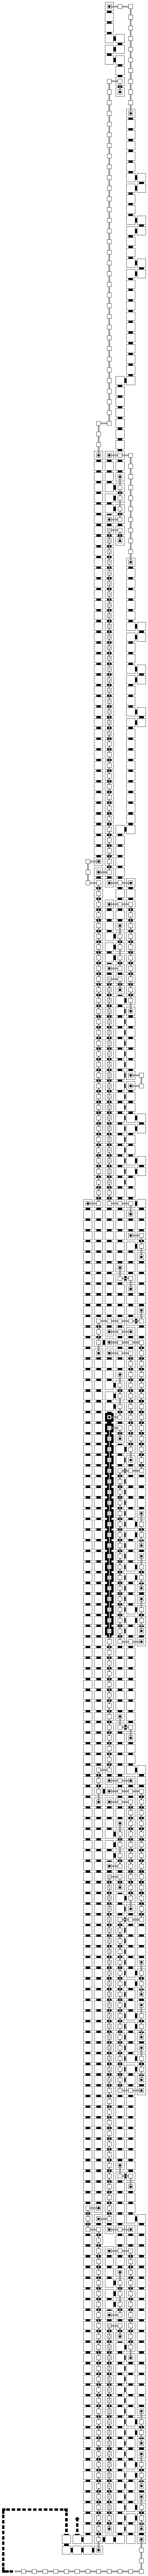
\includegraphics[width=0.45in]{overviews/general/second_warp_1_op}}}%
        ~
        \subcaptionbox{
            Digit 2 - general\\ overview.
            \label{fig:second_warp_2_op_overview}
        }{\makebox[0.24\textwidth][c]{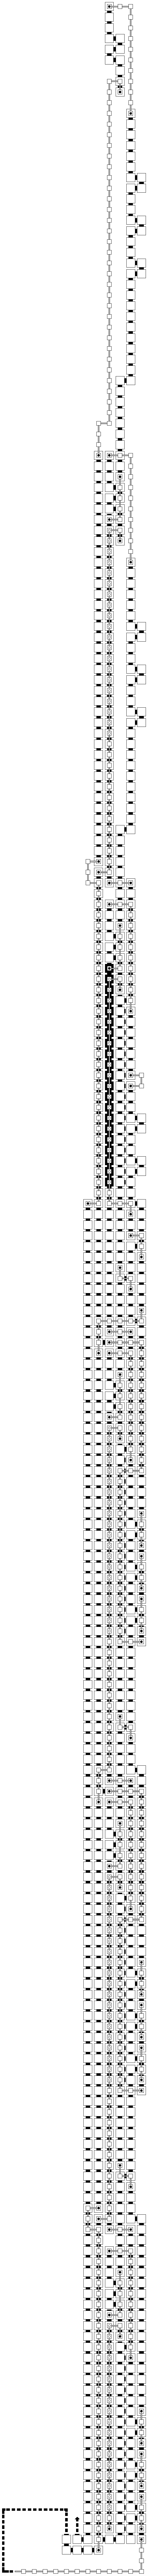
\includegraphics[width=0.45in]{overviews/general/second_warp_2_op}}}%
        ~
        \subcaptionbox{
            Digit 3 - general\\ overview.
            \label{fig:second_warp_3_op_overview}
        }{\makebox[0.24\textwidth][c]{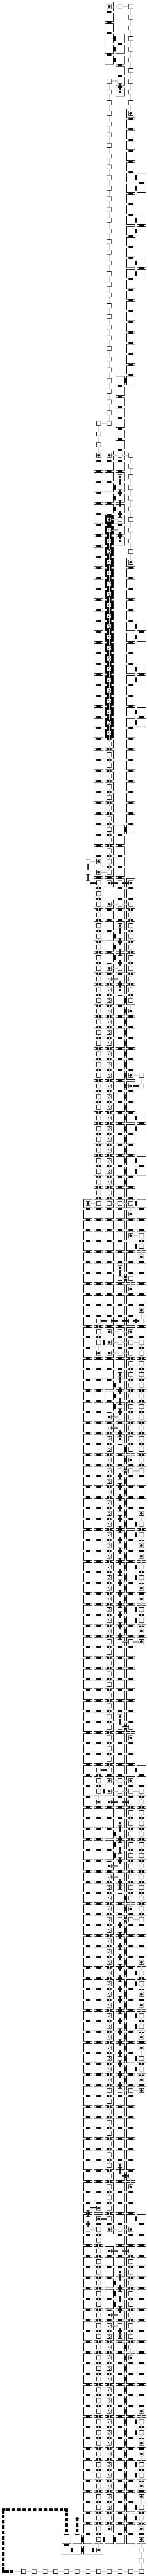
\includegraphics[width=0.45in]{overviews/general/second_warp_3_op}}}%
        ~
        \subcaptionbox{
            Digit 2 - general (seed) overview.
            \label{fig:second_warp_2_seed_op_overview}
        }{\makebox[0.24\textwidth][c]{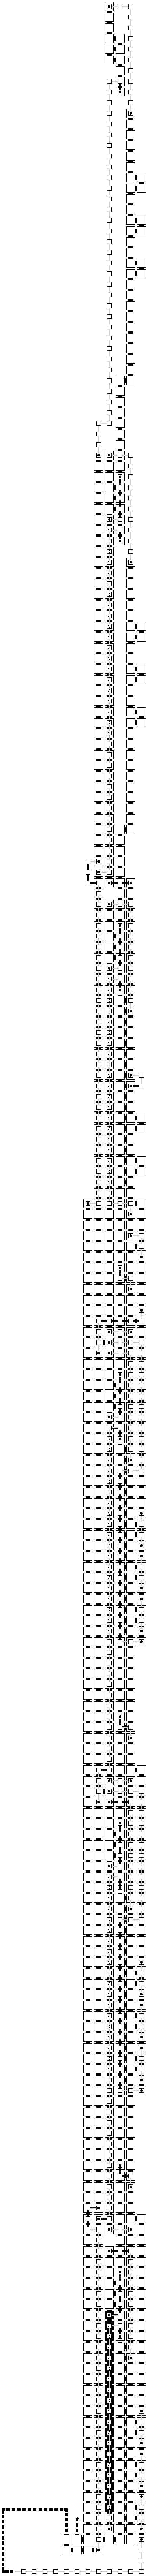
\includegraphics[width=0.45in]{overviews/general/second_warp_2_seed_op}}}%
        ~
    \end{figure}
    \begin{figure}[H]\ContinuedFloat
        \centering
        \subcaptionbox{
            Digit 3 - general (seed) overview.
            \label{fig:second_warp_3_seed_op_overview}
        }{\makebox[0.24\textwidth][c]{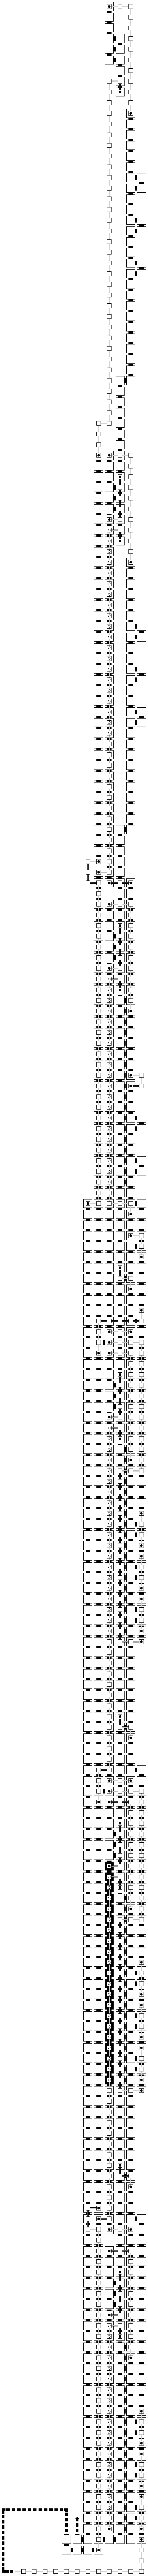
\includegraphics[width=0.45in]{overviews/general/second_warp_3_seed_op}}}%
        ~
        \subcaptionbox{
            Digit 2 - case 2 overview.
            \label{fig:second_warp_2_op_msr_msd_overview}
        }{\makebox[0.24\textwidth][c]{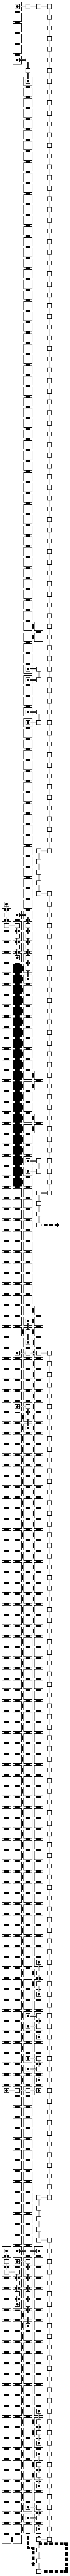
\includegraphics[width=0.45in]{overviews/case2/second_warp_2_op_msr_msd}}}%
        ~
        \subcaptionbox{
            Digit 2 - case 2 (seed) overview.
            \label{fig:second_warp_2_seed_op_msr_msd_overview}
        }{\makebox[0.24\textwidth][c]{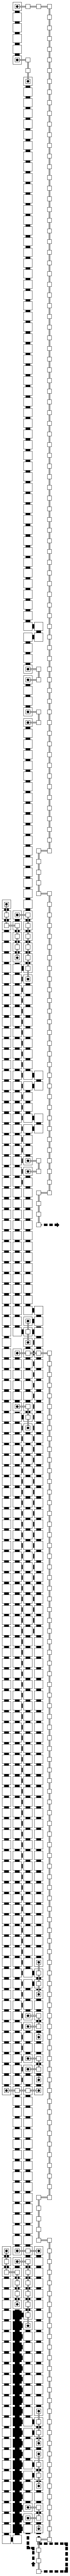
\includegraphics[width=0.45in]{overviews/case2/second_warp_2_seed_op_msr_msd}}}%
        ~
        \subcaptionbox{
            Digit 3 - case 3 overview.
            \label{fig:second_warp_3_op_msr_msd_overview}
        }{\makebox[0.24\textwidth][c]{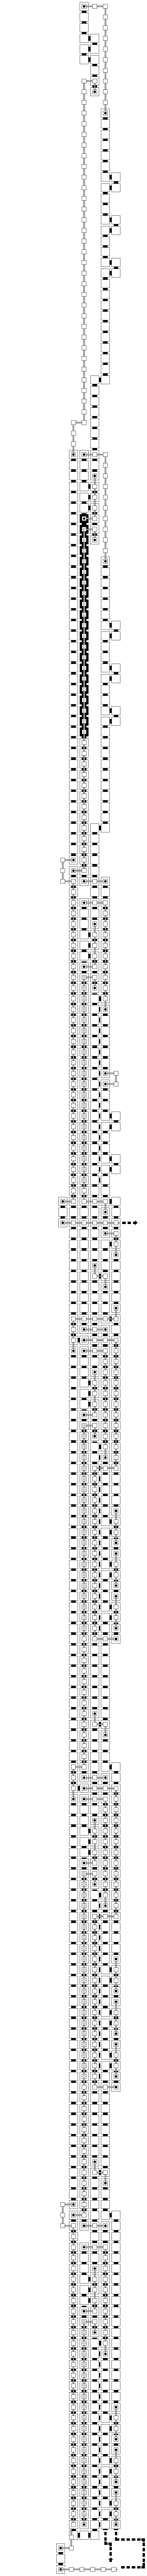
\includegraphics[width=0.45in]{overviews/case3/second_warp_3_op_msr_msd}}}%
        ~
    \end{figure}
    \begin{figure}[H]\ContinuedFloat
        \centering
        \subcaptionbox{
            Digit 3 - case 3 (seed) overview.
            \label{fig:second_warp_3_seed_op_msr_msd_overview}
        }{\makebox[0.24\textwidth][c]{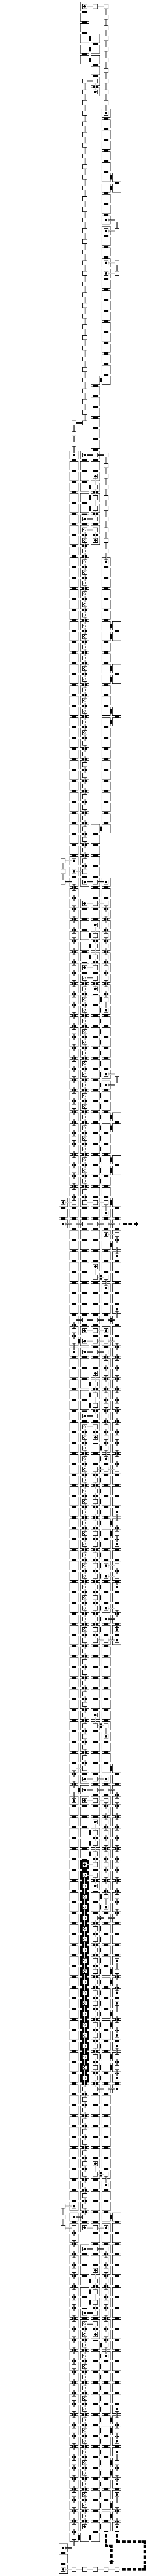
\includegraphics[width=0.45in]{overviews/case3/second_warp_3_seed_op_msr_msd}}}%
        ~
        \caption{\label{fig:second_warp_gadgets_overviews} The {\secondwarp} gadget overviews.}
    \end{figure}


    \item {\postwarp}: \\
    The {\postwarp} gadget is the final gadget to assemble in the {\warpunit}.
    %
    The idea of this gadget is to assemble from wherever the last warping tiles ``wake up'', forming a path that ends where the next digit needs to start being written.
    %
    Since it is the last gadget to assemble in the {\warpunit}, this gadget outputs a signal allowing the {\cwrite} gadgets to assemble to digit that was being passed along.
    %

    For each $i = 1,2,3, u \in \{0, 1\}^l$, and each $\inc \in \ops$:
    \begin{itemize}
       \item Create
        $\begin{aligned}[t]
            \postwarp(& \left \langle {\tt PostWarp},     i, u, \inc \right\rangle,    % Down
                        \left \langle {\tt CounterWrite}, i, u, \inc \right\rangle \;) % North
        \end{aligned}$ \\
        from the general gadget shown in Figure~\ref{fig:post_warp_1_op} if $i = 1$,
        or Figure~\ref{fig:post_warp_2or3_op} if $ i = 2$ or $i = 3$.
        \vspace{.5cm}


        \item Create
        $\begin{aligned}[t]
            \postwarp(& \left \langle {\tt PostWarp},     1, u, \inc, {\tt msr} \right\rangle,    % West
                        \left \langle {\tt CounterWrite}, 1, u, \inc, {\tt msr} \right\rangle \;) % North
        \end{aligned}$ \\
        from the general gadget in Figure~\ref{fig:post_warp_1_op_msr}.
        \vspace{.5cm}

        \item For each $i=1,2,3$: create\\
        $\begin{aligned}[t]
            \postwarp(& \left \langle {\tt PostWarp},     i, u, \inc, {\tt msr}, {\tt msd} \right\rangle,    % Down if i=1 or i=3, West if i=2
                        \left \langle {\tt CounterWrite}, i, u, \inc, {\tt msr}, {\tt msd} \right\rangle \;) % North
        \end{aligned}$ \\
        from the general gadget shown in Figure~\ref{fig:post_warp_1_op_msr_msd} if $i = 1$, or
        Figure~\ref{fig:post_warp_2_op_msr_msd} if $i = 2$, or Figure~\ref{fig:post_warp_2or3_op} if $i = 3$.
        \vspace{.5cm}
    \end{itemize}

    In this step, for digit 1 in the general case,
    %
    $3 \cdot 2^l \cdot 27 =$
    %
    $81 \cdot 2^l =$
    %
    $81 \cdot 2^{\ceil*{{\log m}} + 2} =$
    %
    $324 \cdot 2^{\ceil*{\log m}} \leq$
    %
    $648 \cdot 2^{\log m} = \bigom$ tiles were created.
    %

    For digits 2 \& 3 in the general case,
    %
    $6 \cdot 2^l \cdot 25 =$
    %
    $150 \cdot 2^l =$
    %
    $150 \cdot 2^{\ceil*{{\log m}} + 2} =$
    %
    $600 \cdot 2^{\ceil*{\log m}} \leq$
    %
    $1200 \cdot 2^{\log m} = \bigom$ tiles were created.
    %

    For digit 1 in case 1,
    %
    $3 \cdot 2^l \cdot 25 =$
    %
    $75 \cdot 2^l =$
    %
    $75 \cdot 2^{\ceil*{{\log m}} + 2} =$
    %
    $300 \cdot 2^{\ceil*{\log m}} \leq$
    %
    $600 \cdot 2^{\log m} = \bigom$ tiles were created.
    %

    For digit 1 in case 2,
    %
    $3 \cdot 2^l \cdot 26 =$
    %
    $78 \cdot 2^l =$
    %
    $78 \cdot 2^{\ceil*{{\log m}} + 2} =$
    %
    $312 \cdot 2^{\ceil*{\log m}} \leq$
    %
    $624 \cdot 2^{\log m} = \bigom$ tiles were created.
    %

    For digit 2 in case 2,
    %
    $3 \cdot 2^l \cdot 22 =$
    %
    $66 \cdot 2^l =$
    %
    $66 \cdot 2^{\ceil*{{\log m}} + 2} =$
    %
    $264 \cdot 2^{\ceil*{\log m}} \leq$
    %
    $528 \cdot 2^{\log m} = \bigom$ tiles were created.
    %

    For digit 3 in case 3,
    %
    $3 \cdot 2^l \cdot 25 =$
    %
    $75 \cdot 2^l =$
    %
    $75 \cdot 2^{\ceil*{{\log m}} + 2} =$
    %
    $300 \cdot 2^{\ceil*{\log m}} \leq$
    %
    $600 \cdot 2^{\log m} = \bigom$ tiles were created.
    %

    \begin{figure}[H]
        \centering
        \subcaptionbox{
            Digit 1 - general. There are 27 tiles in this gadget.
            \label{fig:post_warp_1_op}
        }{\makebox[0.24\textwidth][c]{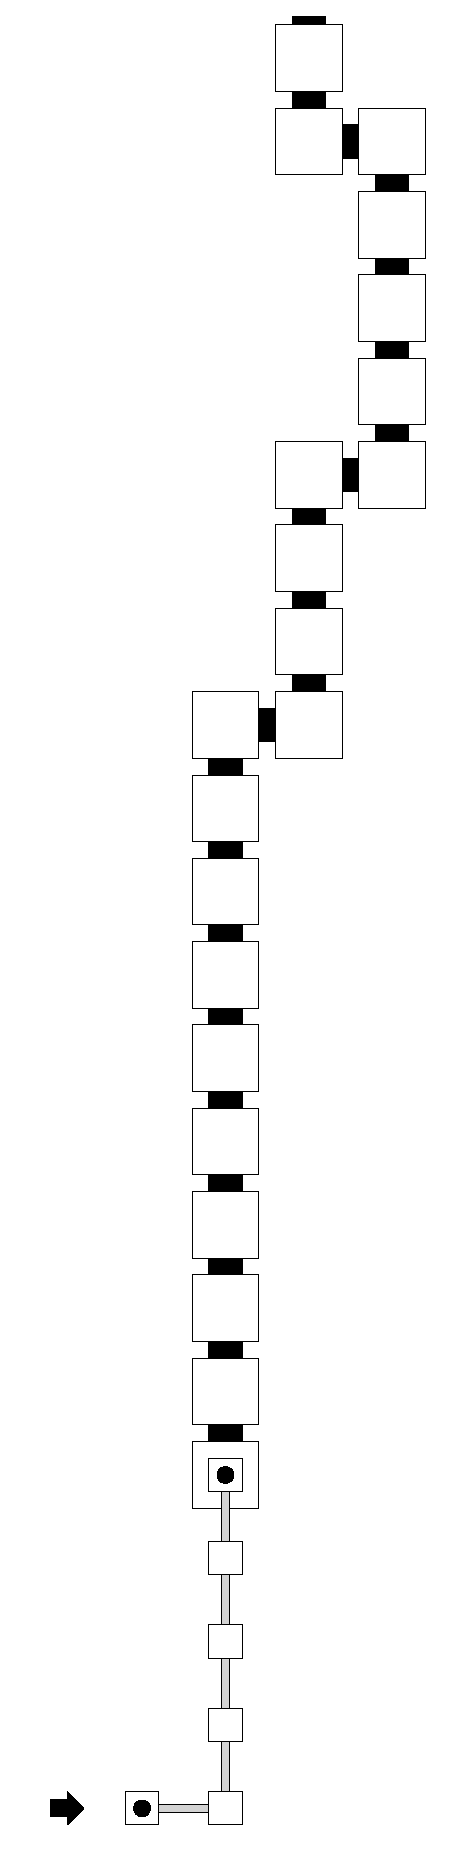
\includegraphics[width=0.45in]{warping_post_warp_general_digit1}}}%
        ~
        \subcaptionbox{
            Digit 1 - general\\overview.
            The black tiles in this figure correspond to the gadget shown in subfigure~\subref{fig:post_warp_1_op}.
            \label{fig:post_warp_1_op_overview}
        }{\makebox[0.24\textwidth][c]{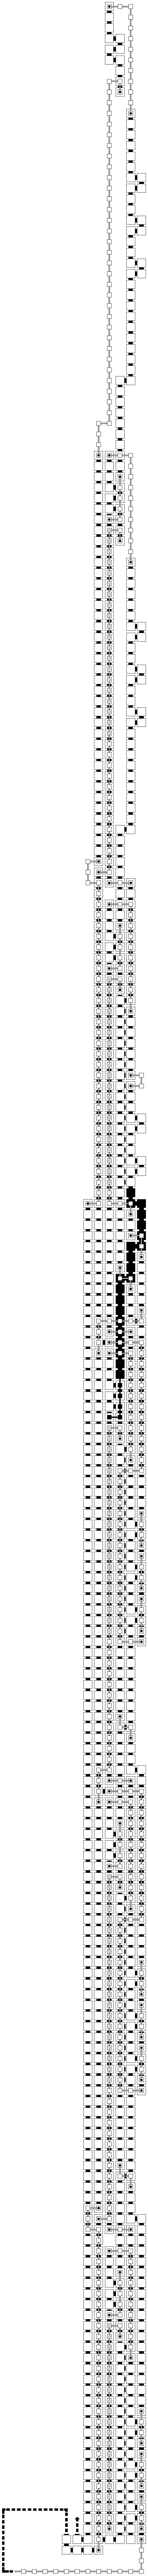
\includegraphics[width=0.45in]{overviews/general/post_warp_1_op}}}%
        ~
        \subcaptionbox{
            Digit 2 \& 3 - general, digit 3 - case 3. There are 25 tiles in this gadget.
            \label{fig:post_warp_2or3_op}
        }{\makebox[0.24\textwidth][c]{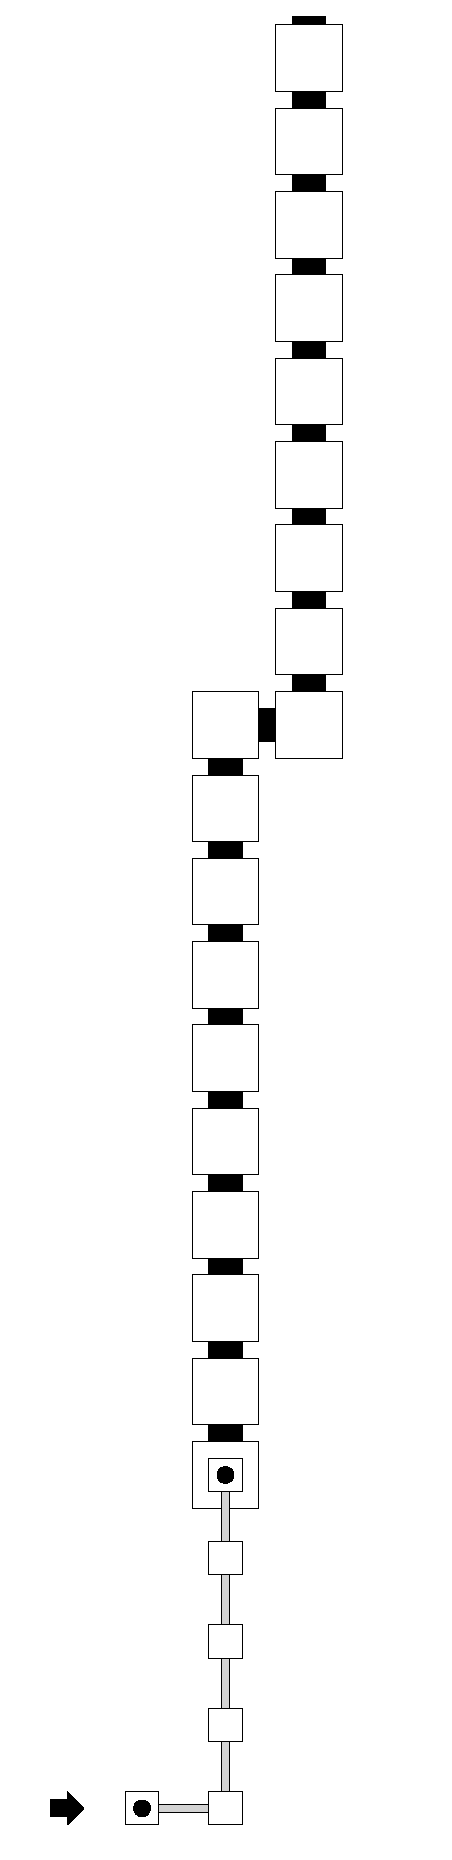
\includegraphics[width=0.45in]{warping_post_warp_general_digit2and3}}}%
        ~
        \subcaptionbox{
            Digit 2 - general\\overview.
            The black tiles in this figure correspond to the gadget shown in subfigure~\subref{fig:post_warp_2or3_op}.
            \label{fig:post_warp_2_op_overview}
        }{\makebox[0.24\textwidth][c]{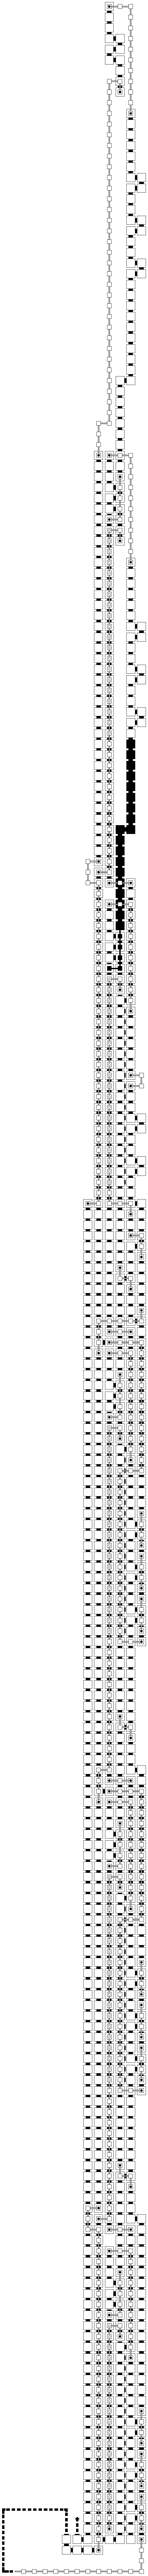
\includegraphics[width=0.45in]{overviews/general/post_warp_2_op}}}%
        ~
    \end{figure}
    \begin{figure}[H]\ContinuedFloat
        \centering
        \subcaptionbox{
            Digit 2 - general (seed) overview.
            The black tiles in this figure correspond to the gadget shown in subfigure~\subref{fig:post_warp_2or3_op}.
            \label{fig:post_warp_2_seed_op_overview}
        }{\makebox[0.24\textwidth][c]{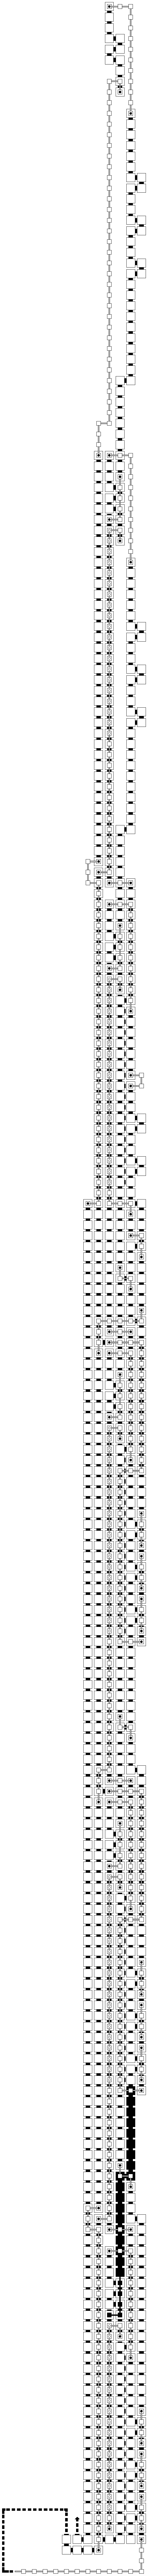
\includegraphics[width=0.45in]{overviews/general/post_warp_2_seed_op}}}%
        ~
        \subcaptionbox{
            Digit 3 - general\\overview.
            The black tiles in this figure correspond to the gadget shown in subfigure~\subref{fig:post_warp_2or3_op}.
            \label{fig:post_warp_3_op_overview}
        }{\makebox[0.24\textwidth][c]{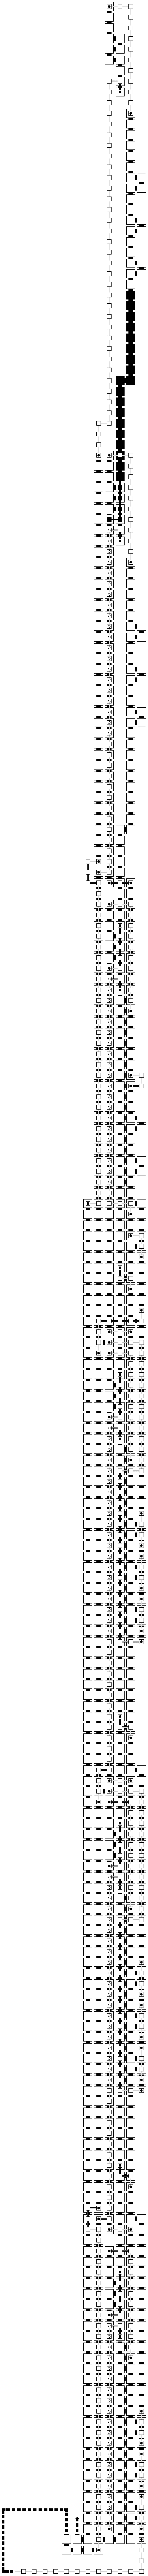
\includegraphics[width=0.45in]{overviews/general/post_warp_3_op}}}%
        ~
        \subcaptionbox{
            Digit 3 - general (seed) overview.
            The black tiles in this figure correspond to the gadget shown in subfigure~\subref{fig:post_warp_2or3_op}.
            \label{fig:post_warp_3_seed_op_overview}
        }{\makebox[0.24\textwidth][c]{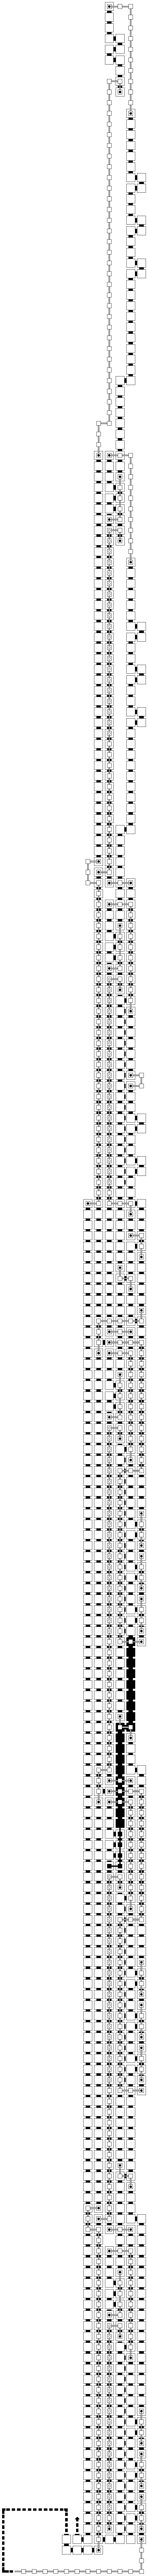
\includegraphics[width=0.45in]{overviews/general/post_warp_3_seed_op}}}%
        ~
        \subcaptionbox{
            Digit 1 - case 1. There are 25 tiles in this gadget.
            \label{fig:post_warp_1_op_msr_msd}
        }{\makebox[0.24\textwidth][c]{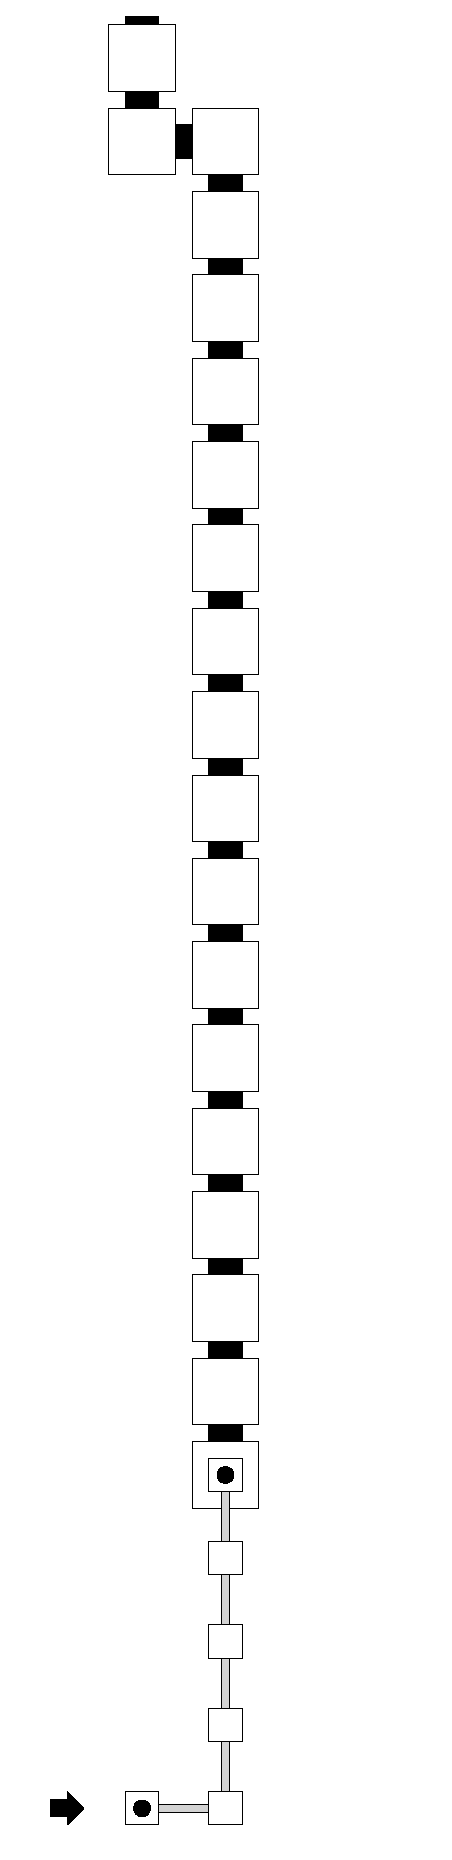
\includegraphics[width=0.45in]{warping_post_warp_case1_digit1_msr}}}%
        ~
    \end{figure}
    \begin{figure}[H]\ContinuedFloat
        \centering
        \subcaptionbox{
            Digit 1 - case 2 overview.
            The black tiles in this figure correspond to the gadget shown in subfigure~\subref{fig:post_warp_1_op_msr_msd}.
            \label{fig:post_warp_1_op_msr_msd_overview}
        }{\makebox[0.24\textwidth][c]{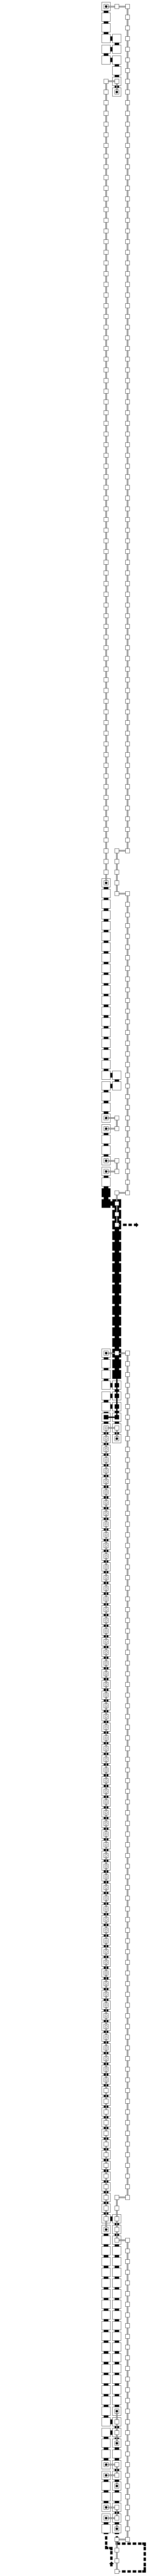
\includegraphics[width=0.45in]{overviews/case1/post_warp_1_op_msr_msd}}}%
        ~
        \subcaptionbox{
            Digit 1 - case 2. There are 26 tiles in this gadget.
            \label{fig:post_warp_1_op_msr}
        }{\makebox[0.24\textwidth][c]{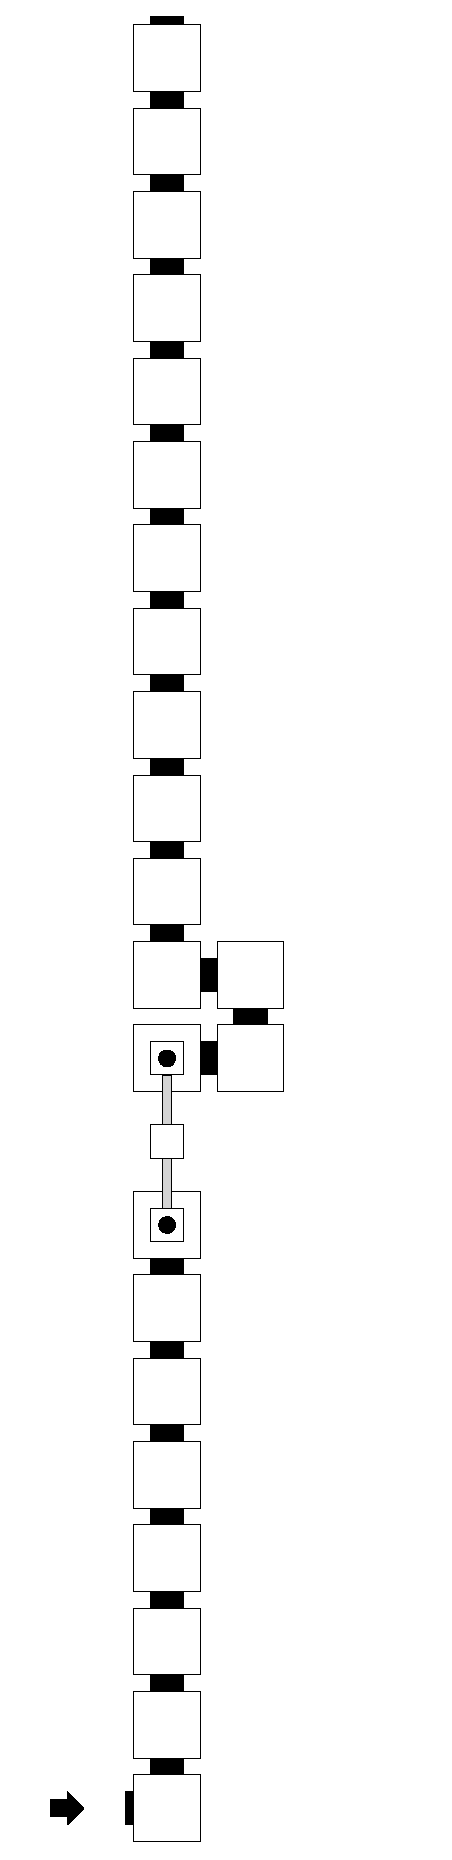
\includegraphics[width=0.45in]{warping_post_warp_case2_digit1_msr}}}%
        ~
        \subcaptionbox{
            Digit 1 - case 2 overview.
            The black tiles in this figure correspond to the gadget shown in subfigure~\subref{fig:post_warp_1_op_msr}.
            \label{fig:post_warp_1_op_msr_overview}
        }{\makebox[0.24\textwidth][c]{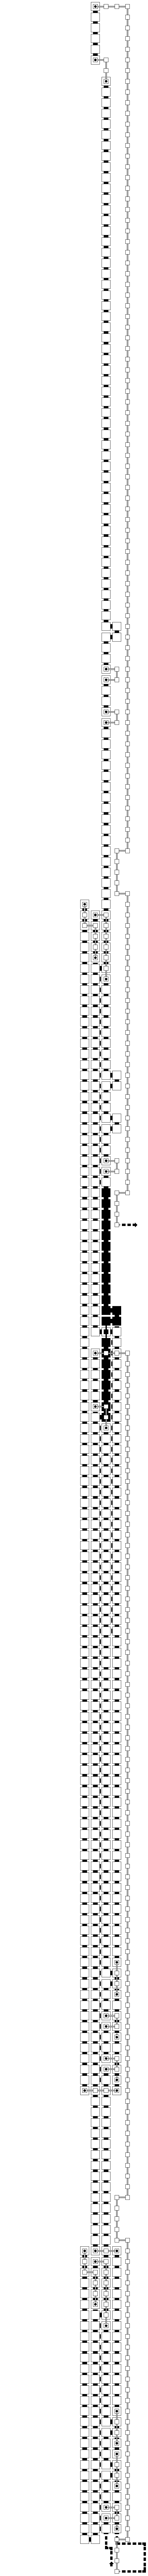
\includegraphics[width=0.45in]{overviews/case2/post_warp_1_op_msr}}}%
        ~
        \subcaptionbox{
            Digit 2 - case 2. There are 22 tiles in this gadget.
            \label{fig:post_warp_2_op_msr_msd}
        }{\makebox[0.24\textwidth][c]{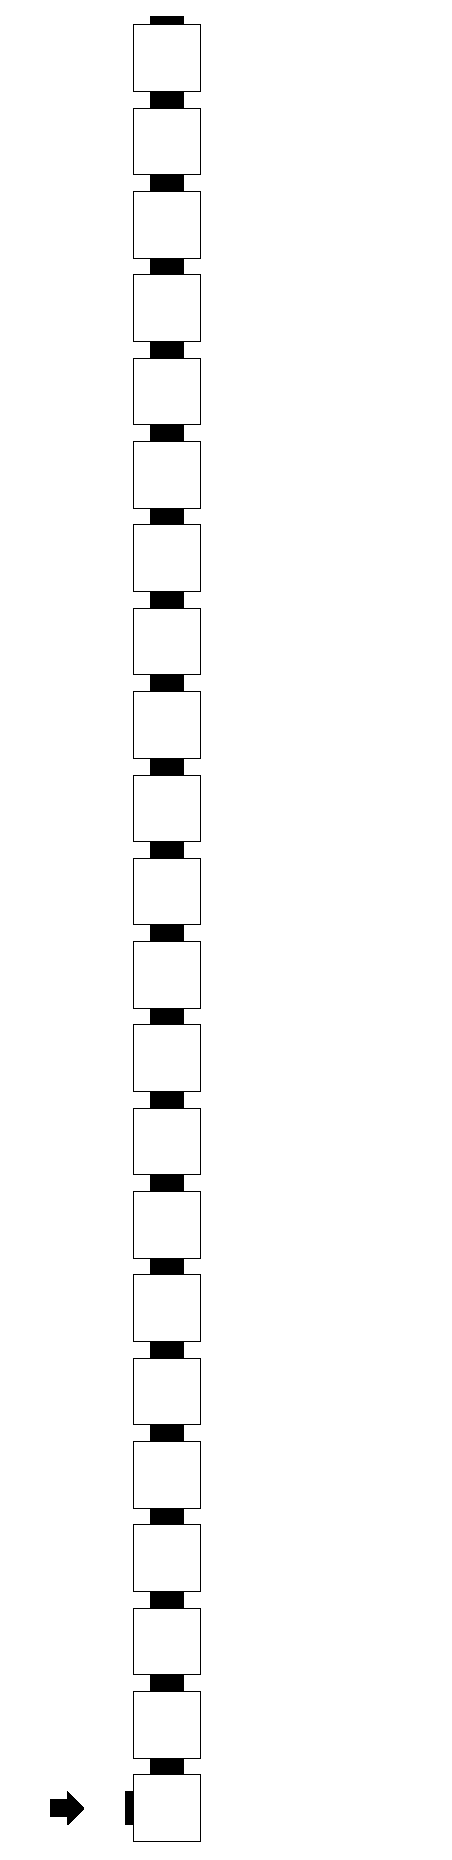
\includegraphics[width=0.45in]{warping_post_warp_case2_digit2_msr}}}%
        ~
    \end{figure}
    \begin{figure}[H]\ContinuedFloat
        \centering
        \subcaptionbox{
            Digit 2 - case 2\\overview.
            The black tiles in this figure correspond to the gadget shown in subfigure~\subref{fig:post_warp_2_op_msr_msd}.
            \label{fig:post_warp_2_op_msr_msd_overview}
        }{\makebox[0.24\textwidth][c]{\includegraphics[width=0.45in]{overviews/case2/post_warp_2_op_msr_msd}}}%
        ~
        \subcaptionbox{
            Digit 2 - case 2 (seed) overview.
            The black tiles in this figure correspond to the gadget shown in subfigure~\subref{fig:post_warp_2_op_msr_msd}.
            \label{fig:post_warp_2_seed_op_msr_msd_overview}
        }{\makebox[0.24\textwidth][c]{\includegraphics[width=0.45in]{overviews/case2/post_warp_2_seed_op_msr_msd}}}%
        ~
        \subcaptionbox{
            Digit 3 - case 3 overview.
            The black tiles in this figure correspond to the gadget shown in subfigure~\subref{fig:post_warp_2or3_op}.
            \label{fig:post_warp_3_op_msr_msd_overview}
        }{\makebox[0.24\textwidth][c]{\includegraphics[width=0.45in]{overviews/case3/post_warp_3_op_msr_msd}}}%
        ~
        \subcaptionbox{
            Digit 3 - case 3 (seed) overview.
            The black tiles in this figure correspond to the gadget shown in subfigure~\subref{fig:post_warp_2or3_op}.
            \label{fig:post_warp_3_seed_op_msr_msd_overview}
        }{\makebox[0.24\textwidth][c]{\includegraphics[width=0.45in]{overviews/case3/post_warp_3_seed_op_msr_msd}}}%
        ~
        \caption{\label{fig:post_warp_gadgets} The {\postwarp} gadgets.}
    \end{figure}
\end{itemize}
